\documentclass[twoside]{book}

% Packages required by doxygen
\usepackage{fixltx2e}
\usepackage{calc}
\usepackage{doxygen}
\usepackage[export]{adjustbox} % also loads graphicx
\usepackage{graphicx}
\usepackage[utf8]{inputenc}
\usepackage{makeidx}
\usepackage{multicol}
\usepackage{multirow}
\PassOptionsToPackage{warn}{textcomp}
\usepackage{textcomp}
\usepackage[nointegrals]{wasysym}
\usepackage[table]{xcolor}

% Font selection
\usepackage[T1]{fontenc}
\usepackage[scaled=.90]{helvet}
\usepackage{courier}
\usepackage{amssymb}
\usepackage{sectsty}
\renewcommand{\familydefault}{\sfdefault}
\allsectionsfont{%
  \fontseries{bc}\selectfont%
  \color{darkgray}%
}
\renewcommand{\DoxyLabelFont}{%
  \fontseries{bc}\selectfont%
  \color{darkgray}%
}
\newcommand{\+}{\discretionary{\mbox{\scriptsize$\hookleftarrow$}}{}{}}

% Page & text layout
\usepackage{geometry}
\geometry{%
  a4paper,%
  top=2.5cm,%
  bottom=2.5cm,%
  left=2.5cm,%
  right=2.5cm%
}
\tolerance=750
\hfuzz=15pt
\hbadness=750
\setlength{\emergencystretch}{15pt}
\setlength{\parindent}{0cm}
\setlength{\parskip}{3ex plus 2ex minus 2ex}
\makeatletter
\renewcommand{\paragraph}{%
  \@startsection{paragraph}{4}{0ex}{-1.0ex}{1.0ex}{%
    \normalfont\normalsize\bfseries\SS@parafont%
  }%
}
\renewcommand{\subparagraph}{%
  \@startsection{subparagraph}{5}{0ex}{-1.0ex}{1.0ex}{%
    \normalfont\normalsize\bfseries\SS@subparafont%
  }%
}
\makeatother

% Headers & footers
\usepackage{fancyhdr}
\pagestyle{fancyplain}
\fancyhead[LE]{\fancyplain{}{\bfseries\thepage}}
\fancyhead[CE]{\fancyplain{}{}}
\fancyhead[RE]{\fancyplain{}{\bfseries\leftmark}}
\fancyhead[LO]{\fancyplain{}{\bfseries\rightmark}}
\fancyhead[CO]{\fancyplain{}{}}
\fancyhead[RO]{\fancyplain{}{\bfseries\thepage}}
\fancyfoot[LE]{\fancyplain{}{}}
\fancyfoot[CE]{\fancyplain{}{}}
\fancyfoot[RE]{\fancyplain{}{\bfseries\scriptsize Generated by Doxygen }}
\fancyfoot[LO]{\fancyplain{}{\bfseries\scriptsize Generated by Doxygen }}
\fancyfoot[CO]{\fancyplain{}{}}
\fancyfoot[RO]{\fancyplain{}{}}
\renewcommand{\footrulewidth}{0.4pt}
\renewcommand{\chaptermark}[1]{%
  \markboth{#1}{}%
}
\renewcommand{\sectionmark}[1]{%
  \markright{\thesection\ #1}%
}

% Indices & bibliography
\usepackage{natbib}
\usepackage[titles]{tocloft}
\setcounter{tocdepth}{3}
\setcounter{secnumdepth}{5}
\makeindex

% Hyperlinks (required, but should be loaded last)
\usepackage{ifpdf}
\ifpdf
  \usepackage[pdftex,pagebackref=true]{hyperref}
\else
  \usepackage[ps2pdf,pagebackref=true]{hyperref}
\fi
\hypersetup{%
  colorlinks=true,%
  linkcolor=blue,%
  citecolor=blue,%
  unicode%
}

% Custom commands
\newcommand{\clearemptydoublepage}{%
  \newpage{\pagestyle{empty}\cleardoublepage}%
}

\usepackage{caption}
\captionsetup{labelsep=space,justification=centering,font={bf},singlelinecheck=off,skip=4pt,position=top}

%===== C O N T E N T S =====

\begin{document}

% Titlepage & ToC
\hypersetup{pageanchor=false,
             bookmarksnumbered=true,
             pdfencoding=unicode
            }
\pagenumbering{alph}
\begin{titlepage}
\vspace*{7cm}
\begin{center}%
{\Large I\+CP Project \\[1ex]\large 0.\+1 }\\
\vspace*{1cm}
{\large Generated by Doxygen 1.8.13}\\
\end{center}
\end{titlepage}
\clearemptydoublepage
\pagenumbering{roman}
\tableofcontents
\clearemptydoublepage
\pagenumbering{arabic}
\hypersetup{pageanchor=true}

%--- Begin generated contents ---
\chapter{I\+C\+P\+Proj}
\label{md_README}
\Hypertarget{md_README}
\input{md_README}
\chapter{Hierarchical Index}
\section{Class Hierarchy}
This inheritance list is sorted roughly, but not completely, alphabetically\+:\begin{DoxyCompactList}
\item \contentsline{section}{Drawable\+Object}{\pageref{classDrawableObject}}{}
\begin{DoxyCompactList}
\item \contentsline{section}{Block}{\pageref{classBlock}}{}
\item \contentsline{section}{Link}{\pageref{classLink}}{}
\item \contentsline{section}{Port}{\pageref{classPort}}{}
\end{DoxyCompactList}
\item \contentsline{section}{Load\+Manager}{\pageref{classLoadManager}}{}
\item \contentsline{section}{Point2D}{\pageref{classPoint2D}}{}
\item Q\+Dialog\begin{DoxyCompactList}
\item \contentsline{section}{Block\+Dialog}{\pageref{classBlockDialog}}{}
\end{DoxyCompactList}
\item Q\+Rect\begin{DoxyCompactList}
\item \contentsline{section}{My\+Rect}{\pageref{classMyRect}}{}
\end{DoxyCompactList}
\item Q\+Widget\begin{DoxyCompactList}
\item \contentsline{section}{Widget}{\pageref{classWidget}}{}
\end{DoxyCompactList}
\end{DoxyCompactList}

\chapter{Class Index}
\section{Class List}
Here are the classes, structs, unions and interfaces with brief descriptions\+:\begin{DoxyCompactList}
\item\contentsline{section}{\hyperlink{classBlock}{Block} }{\pageref{classBlock}}{}
\item\contentsline{section}{\hyperlink{classBlockDialog}{Block\+Dialog} }{\pageref{classBlockDialog}}{}
\item\contentsline{section}{\hyperlink{classDrawableObject}{Drawable\+Object} }{\pageref{classDrawableObject}}{}
\item\contentsline{section}{\hyperlink{classLink}{Link} }{\pageref{classLink}}{}
\item\contentsline{section}{\hyperlink{classLoadManager}{Load\+Manager} }{\pageref{classLoadManager}}{}
\item\contentsline{section}{\hyperlink{classMyRect}{My\+Rect} }{\pageref{classMyRect}}{}
\item\contentsline{section}{\hyperlink{classPoint2D}{Point2D} }{\pageref{classPoint2D}}{}
\item\contentsline{section}{\hyperlink{classPort}{Port} }{\pageref{classPort}}{}
\item\contentsline{section}{\hyperlink{classWidget}{Widget} }{\pageref{classWidget}}{}
\end{DoxyCompactList}

\chapter{Class Documentation}
\hypertarget{classBlock}{}\section{Block Class Reference}
\label{classBlock}\index{Block@{Block}}
Inheritance diagram for Block\+:\begin{figure}[H]
\begin{center}
\leavevmode
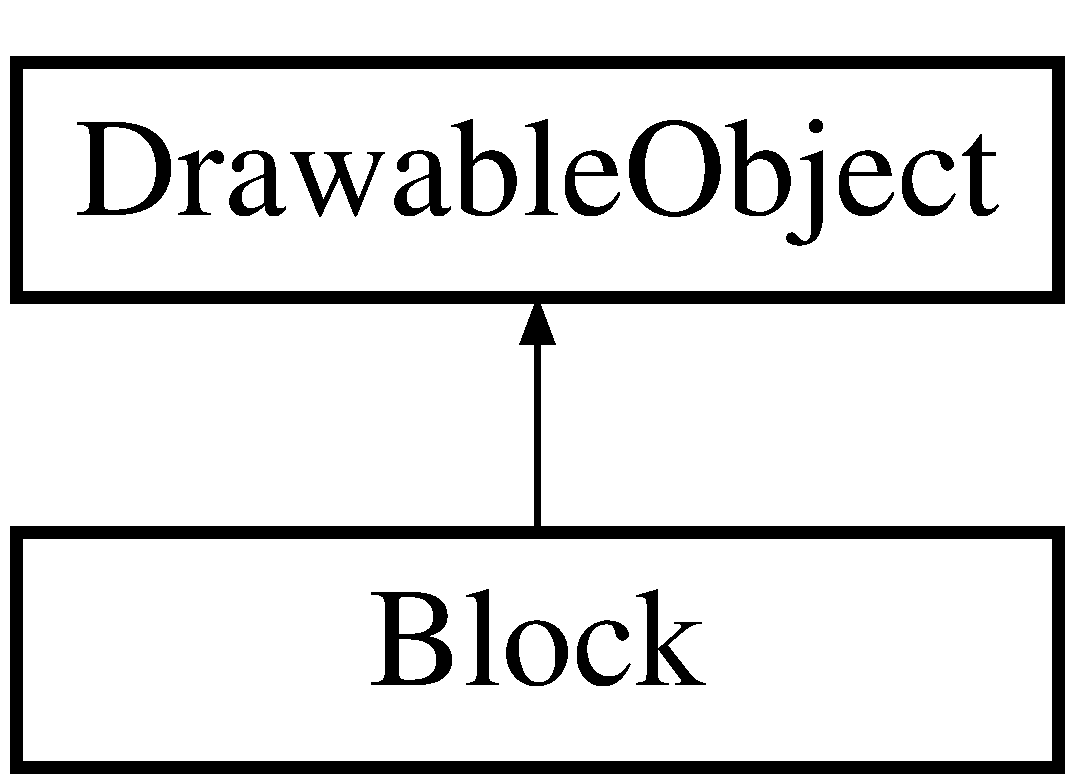
\includegraphics[height=2.000000cm]{classBlock}
\end{center}
\end{figure}
\subsection*{Public Member Functions}
\begin{DoxyCompactItemize}
\item 
\hyperlink{classBlock_a323497a43c8db217fce86704990008c9}{Block} (E\+Block e\+Block, \hyperlink{classMyRect}{My\+Rect} $\ast$rect)
\item 
\hyperlink{classBlock_a36a6f635930ffe1ba55af52236e911dd}{Block} (E\+Block e\+Block, \hyperlink{classMyRect}{My\+Rect} $\ast$rect, double \hyperlink{classBlock_afb64e6479c44387ece15c0f8d635236f}{value})
\item 
void \hyperlink{classBlock_a1a02b48229dc2df1d58b1c7a202f3e5e}{gen\+In\+Port} ()
\item 
std\+::vector$<$ \hyperlink{classPort}{Port} $\ast$ $>$ \hyperlink{classBlock_af10d358559032e920b7b8ad25c113b69}{get\+In\+Ports} ()
\item 
\hyperlink{classPort}{Port} $\ast$ \hyperlink{classBlock_a897dd6edfbdec3930d764aa39f0d3de8}{get\+Out\+Port} ()
\item 
void \hyperlink{classBlock_a82671bfde9a0d710c72ef5004fdb4179}{set\+Out\+Port} (\hyperlink{classPort}{Port} $\ast$p)
\item 
void \hyperlink{classBlock_aa67c1224df9015c055fa5523dfa67f52}{set\+In\+Ports} (std\+::vector$<$ \hyperlink{classPort}{Port} $\ast$$>$ portvector)
\item 
void \hyperlink{classBlock_aa24819f99f922d0b2cba3d12775974e0}{set\+In\+Port} (int index, \hyperlink{classPort}{Port} $\ast$new\+In\+Port)
\item 
double \hyperlink{classBlock_a613dd5c447f2a2dccebdaba7c2b4b74c}{get\+Value} () const
\item 
void \hyperlink{classBlock_acabb5bf7f41bc16338b4efde5a760703}{set\+Value} (double \hyperlink{classBlock_afb64e6479c44387ece15c0f8d635236f}{value})
\item 
\hyperlink{classMyRect}{My\+Rect} $\ast$ \hyperlink{classBlock_ad4c55f893fad7eec6e2ecaa9e6bec6da}{get\+Resize\+Rect} ()
\item 
E\+Block \hyperlink{classBlock_aefadce64bb60ab2e12a23bce510b74da}{get\+Type} () const
\item 
void \hyperlink{classBlock_a939528c280e4d7f516422f85bb22c2d2}{set\+Rect\+Position} (\hyperlink{classPoint2D}{Point2D} $\ast$position)
\item 
\hyperlink{classMyRect}{My\+Rect} $\ast$ \hyperlink{classBlock_a396f46a4f7592ffdf4d168be2e79ee52}{get\+Rect} () const
\item 
void \hyperlink{classBlock_a0ee328fa6748cad1232dd0803710dbf0}{set\+Rect} (\hyperlink{classMyRect}{My\+Rect} $\ast$rect)
\item 
void \hyperlink{classBlock_a931b0465363ea2ec445f817940a78abd}{set\+Type} (E\+Block e\+Block)
\item 
void \hyperlink{classBlock_a6e2da20e7645ed07ff449256fc2cc767}{Move} (\hyperlink{classPoint2D}{Point2D} $\ast$delta)
\item 
void \hyperlink{classBlock_a88a3549580bb9504230921c8d10ca9dd}{Resize} (\hyperlink{classPoint2D}{Point2D} $\ast$)
\item 
virtual void \hyperlink{classBlock_a3561d9ce6a8eee10ca8c397e3d25dc5c}{Draw} (Q\+Painter $\ast$painter) override
\item 
bool \hyperlink{classBlock_a5429186079cf37c2b09fef7d377f8a28}{complete\+Delete\+Block} ()
\end{DoxyCompactItemize}
\subsection*{Static Public Member Functions}
\begin{DoxyCompactItemize}
\item 
static bool \hyperlink{classBlock_aafbf3dd9d1af0a328878662cceb7de26}{is\+Cycled} (\hyperlink{classBlock}{Block} $\ast$comparing, \hyperlink{classBlock}{Block} $\ast$block)
\item 
static double \hyperlink{classBlock_a801eecced930d343cd4cd5fa14068be1}{compute} (\hyperlink{classBlock}{Block} $\ast$block)
\item 
static void \hyperlink{classBlock_ab76d443f7898f82c4ad4cb124375a76c}{unset\+Calculated} (\hyperlink{classBlock}{Block} $\ast$block)
\end{DoxyCompactItemize}
\subsection*{Static Public Attributes}
\begin{DoxyCompactItemize}
\item 
static const int \hyperlink{classBlock_ab2e1f1dd232266b80299979e4e3ff4a7}{M\+I\+N\+B\+L\+O\+C\+K\+S\+I\+ZE} = 100
\item 
static const int \hyperlink{classBlock_a968c9b7c94b49e5185f8e490c60fbfc0}{M\+A\+X\+B\+L\+O\+C\+K\+S\+I\+ZE} = 400
\item 
static int \hyperlink{classBlock_acf7c29d2194e317f2cc831046ec5460e}{step\+Counter}
\end{DoxyCompactItemize}
\subsection*{Private Member Functions}
\begin{DoxyCompactItemize}
\item 
void \hyperlink{classBlock_a4f7dbdad50f95ab979cfdb86c4b63018}{calculate\+Ports\+To\+Middle} ()
\item 
bool \hyperlink{classBlock_a3d65e76b1404d38e68243e50034d5551}{recalculate\+Heights} ()
\end{DoxyCompactItemize}
\subsection*{Private Attributes}
\begin{DoxyCompactItemize}
\item 
E\+Block \hyperlink{classBlock_a2078fc6dc0ee457f3332a38685fea0af}{\+\_\+e\+Block}
\item 
\hyperlink{classMyRect}{My\+Rect} $\ast$ \hyperlink{classBlock_a310ce3c87df1c29e3bfa15aafb9b21c0}{\+\_\+rect} = nullptr
\item 
\hyperlink{classMyRect}{My\+Rect} $\ast$ \hyperlink{classBlock_ae7f260f0bdfd696d33b758a68de30d4c}{\+\_\+resize\+Rect} = nullptr
\item 
Q\+Image \hyperlink{classBlock_aab61fd446868e41197a55c79dc7d709b}{image}
\item 
std\+::vector$<$ \hyperlink{classPort}{Port} $\ast$ $>$ \hyperlink{classBlock_a2b9ee38ee6794399262907587010ed3d}{in\+Ports} = std\+::vector$<$\hyperlink{classPort}{Port}$\ast$$>$()
\item 
\hyperlink{classPort}{Port} $\ast$ \hyperlink{classBlock_a07a89d0108abe2b1ab8b69aabe815d73}{\+\_\+out\+Port} = nullptr
\item 
double \hyperlink{classBlock_afb64e6479c44387ece15c0f8d635236f}{value} = 0
\item 
bool \hyperlink{classBlock_a78ba2fc9a1343e5d9f6f372888e90bf2}{calculated} = false
\item 
Q\+Label $\ast$ \hyperlink{classBlock_a1d3b391e9531eb8bc0b0362730d4c53d}{disp}
\end{DoxyCompactItemize}
\subsection*{Static Private Attributes}
\begin{DoxyCompactItemize}
\item 
static \hyperlink{classBlock}{Block} $\ast$ \hyperlink{classBlock_aad15dd9091823b114a17df309bd68bf4}{debug} = nullptr
\end{DoxyCompactItemize}


\subsection{Constructor \& Destructor Documentation}
\mbox{\Hypertarget{classBlock_a323497a43c8db217fce86704990008c9}\label{classBlock_a323497a43c8db217fce86704990008c9}} 
\index{Block@{Block}!Block@{Block}}
\index{Block@{Block}!Block@{Block}}
\subsubsection{\texorpdfstring{Block()}{Block()}\hspace{0.1cm}{\footnotesize\ttfamily [1/2]}}
{\footnotesize\ttfamily Block\+::\+Block (\begin{DoxyParamCaption}\item[{E\+Block}]{e\+Block,  }\item[{\hyperlink{classMyRect}{My\+Rect} $\ast$}]{rect }\end{DoxyParamCaption})}


\begin{DoxyParams}{Parameters}
{\em e\+Block} & type of the block \\
\hline
{\em rect} & graphic properties of the block \\
\hline
\end{DoxyParams}
\mbox{\Hypertarget{classBlock_a36a6f635930ffe1ba55af52236e911dd}\label{classBlock_a36a6f635930ffe1ba55af52236e911dd}} 
\index{Block@{Block}!Block@{Block}}
\index{Block@{Block}!Block@{Block}}
\subsubsection{\texorpdfstring{Block()}{Block()}\hspace{0.1cm}{\footnotesize\ttfamily [2/2]}}
{\footnotesize\ttfamily Block\+::\+Block (\begin{DoxyParamCaption}\item[{E\+Block}]{e\+Block,  }\item[{\hyperlink{classMyRect}{My\+Rect} $\ast$}]{rect,  }\item[{double}]{value }\end{DoxyParamCaption})}


\begin{DoxyParams}{Parameters}
{\em e\+Block} & type of the block \\
\hline
{\em rect} & graphic properties of the block \\
\hline
{\em value} & internal value of block used by input block \\
\hline
\end{DoxyParams}


\subsection{Member Function Documentation}
\mbox{\Hypertarget{classBlock_a4f7dbdad50f95ab979cfdb86c4b63018}\label{classBlock_a4f7dbdad50f95ab979cfdb86c4b63018}} 
\index{Block@{Block}!calculate\+Ports\+To\+Middle@{calculate\+Ports\+To\+Middle}}
\index{calculate\+Ports\+To\+Middle@{calculate\+Ports\+To\+Middle}!Block@{Block}}
\subsubsection{\texorpdfstring{calculate\+Ports\+To\+Middle()}{calculatePortsToMiddle()}}
{\footnotesize\ttfamily void Block\+::calculate\+Ports\+To\+Middle (\begin{DoxyParamCaption}{ }\end{DoxyParamCaption})\hspace{0.3cm}{\ttfamily [private]}}

Centers input ports in the block. \mbox{\Hypertarget{classBlock_a5429186079cf37c2b09fef7d377f8a28}\label{classBlock_a5429186079cf37c2b09fef7d377f8a28}} 
\index{Block@{Block}!complete\+Delete\+Block@{complete\+Delete\+Block}}
\index{complete\+Delete\+Block@{complete\+Delete\+Block}!Block@{Block}}
\subsubsection{\texorpdfstring{complete\+Delete\+Block()}{completeDeleteBlock()}}
{\footnotesize\ttfamily bool Block\+::complete\+Delete\+Block (\begin{DoxyParamCaption}{ }\end{DoxyParamCaption})}

Calls destructor on block. Deletes \hyperlink{classBlock}{Block} including all its ports and links. \mbox{\Hypertarget{classBlock_a801eecced930d343cd4cd5fa14068be1}\label{classBlock_a801eecced930d343cd4cd5fa14068be1}} 
\index{Block@{Block}!compute@{compute}}
\index{compute@{compute}!Block@{Block}}
\subsubsection{\texorpdfstring{compute()}{compute()}}
{\footnotesize\ttfamily double Block\+::compute (\begin{DoxyParamCaption}\item[{\hyperlink{classBlock}{Block} $\ast$}]{block }\end{DoxyParamCaption})\hspace{0.3cm}{\ttfamily [static]}}

Recursive block calculation from root.

Recursively calls all blocks on all input ports and calculates its values. 
\begin{DoxyParams}{Parameters}
{\em block} & root block to be calculated \\
\hline
\end{DoxyParams}
\begin{DoxyReturn}{Returns}
value of given root block 
\end{DoxyReturn}
\mbox{\Hypertarget{classBlock_a3561d9ce6a8eee10ca8c397e3d25dc5c}\label{classBlock_a3561d9ce6a8eee10ca8c397e3d25dc5c}} 
\index{Block@{Block}!Draw@{Draw}}
\index{Draw@{Draw}!Block@{Block}}
\subsubsection{\texorpdfstring{Draw()}{Draw()}}
{\footnotesize\ttfamily void Block\+::\+Draw (\begin{DoxyParamCaption}\item[{Q\+Painter $\ast$}]{painter }\end{DoxyParamCaption})\hspace{0.3cm}{\ttfamily [override]}, {\ttfamily [virtual]}}

Draws block by Q\+Painter. 
\begin{DoxyParams}{Parameters}
{\em painter} & the pane \\
\hline
\end{DoxyParams}
\begin{DoxySeeAlso}{See also}
Graphics.\+Drawable\+Object\+::\+Draw(\+Q\+Painter$\ast$) 
\end{DoxySeeAlso}


Reimplemented from \hyperlink{classDrawableObject}{Drawable\+Object}.

\mbox{\Hypertarget{classBlock_a1a02b48229dc2df1d58b1c7a202f3e5e}\label{classBlock_a1a02b48229dc2df1d58b1c7a202f3e5e}} 
\index{Block@{Block}!gen\+In\+Port@{gen\+In\+Port}}
\index{gen\+In\+Port@{gen\+In\+Port}!Block@{Block}}
\subsubsection{\texorpdfstring{gen\+In\+Port()}{genInPort()}}
{\footnotesize\ttfamily void Block\+::gen\+In\+Port (\begin{DoxyParamCaption}{ }\end{DoxyParamCaption})}

Generates one input port.

calls \hyperlink{}{Calculate\+Ports\+To\+Middle()} \mbox{\Hypertarget{classBlock_af10d358559032e920b7b8ad25c113b69}\label{classBlock_af10d358559032e920b7b8ad25c113b69}} 
\index{Block@{Block}!get\+In\+Ports@{get\+In\+Ports}}
\index{get\+In\+Ports@{get\+In\+Ports}!Block@{Block}}
\subsubsection{\texorpdfstring{get\+In\+Ports()}{getInPorts()}}
{\footnotesize\ttfamily std\+::vector$<$ \hyperlink{classPort}{Port} $\ast$ $>$ Block\+::get\+In\+Ports (\begin{DoxyParamCaption}{ }\end{DoxyParamCaption})}

Gets the input ports.

\begin{DoxyReturn}{Returns}
the input ports 
\end{DoxyReturn}
\mbox{\Hypertarget{classBlock_a897dd6edfbdec3930d764aa39f0d3de8}\label{classBlock_a897dd6edfbdec3930d764aa39f0d3de8}} 
\index{Block@{Block}!get\+Out\+Port@{get\+Out\+Port}}
\index{get\+Out\+Port@{get\+Out\+Port}!Block@{Block}}
\subsubsection{\texorpdfstring{get\+Out\+Port()}{getOutPort()}}
{\footnotesize\ttfamily \hyperlink{classPort}{Port} $\ast$ Block\+::get\+Out\+Port (\begin{DoxyParamCaption}{ }\end{DoxyParamCaption})}

Gets the output port.

\begin{DoxyReturn}{Returns}
the output port 
\end{DoxyReturn}
\mbox{\Hypertarget{classBlock_a396f46a4f7592ffdf4d168be2e79ee52}\label{classBlock_a396f46a4f7592ffdf4d168be2e79ee52}} 
\index{Block@{Block}!get\+Rect@{get\+Rect}}
\index{get\+Rect@{get\+Rect}!Block@{Block}}
\subsubsection{\texorpdfstring{get\+Rect()}{getRect()}}
{\footnotesize\ttfamily \hyperlink{classMyRect}{My\+Rect} $\ast$ Block\+::get\+Rect (\begin{DoxyParamCaption}{ }\end{DoxyParamCaption}) const}

Gets the rectangle.

\begin{DoxyReturn}{Returns}
the rectangle 
\end{DoxyReturn}
\mbox{\Hypertarget{classBlock_ad4c55f893fad7eec6e2ecaa9e6bec6da}\label{classBlock_ad4c55f893fad7eec6e2ecaa9e6bec6da}} 
\index{Block@{Block}!get\+Resize\+Rect@{get\+Resize\+Rect}}
\index{get\+Resize\+Rect@{get\+Resize\+Rect}!Block@{Block}}
\subsubsection{\texorpdfstring{get\+Resize\+Rect()}{getResizeRect()}}
{\footnotesize\ttfamily \hyperlink{classMyRect}{My\+Rect} $\ast$ Block\+::get\+Resize\+Rect (\begin{DoxyParamCaption}{ }\end{DoxyParamCaption})}

Gets the resizing rectangle.

\begin{DoxyReturn}{Returns}
the rectangle 
\end{DoxyReturn}
\mbox{\Hypertarget{classBlock_aefadce64bb60ab2e12a23bce510b74da}\label{classBlock_aefadce64bb60ab2e12a23bce510b74da}} 
\index{Block@{Block}!get\+Type@{get\+Type}}
\index{get\+Type@{get\+Type}!Block@{Block}}
\subsubsection{\texorpdfstring{get\+Type()}{getType()}}
{\footnotesize\ttfamily E\+Block Block\+::get\+Type (\begin{DoxyParamCaption}{ }\end{DoxyParamCaption}) const}

Gets the type.

\begin{DoxyReturn}{Returns}
the type 
\end{DoxyReturn}
\mbox{\Hypertarget{classBlock_a613dd5c447f2a2dccebdaba7c2b4b74c}\label{classBlock_a613dd5c447f2a2dccebdaba7c2b4b74c}} 
\index{Block@{Block}!get\+Value@{get\+Value}}
\index{get\+Value@{get\+Value}!Block@{Block}}
\subsubsection{\texorpdfstring{get\+Value()}{getValue()}}
{\footnotesize\ttfamily double Block\+::get\+Value (\begin{DoxyParamCaption}{ }\end{DoxyParamCaption}) const}

Gets the value.

\begin{DoxyReturn}{Returns}
the value 
\end{DoxyReturn}
\mbox{\Hypertarget{classBlock_aafbf3dd9d1af0a328878662cceb7de26}\label{classBlock_aafbf3dd9d1af0a328878662cceb7de26}} 
\index{Block@{Block}!is\+Cycled@{is\+Cycled}}
\index{is\+Cycled@{is\+Cycled}!Block@{Block}}
\subsubsection{\texorpdfstring{is\+Cycled()}{isCycled()}}
{\footnotesize\ttfamily bool Block\+::is\+Cycled (\begin{DoxyParamCaption}\item[{\hyperlink{classBlock}{Block} $\ast$}]{comparing,  }\item[{\hyperlink{classBlock}{Block} $\ast$}]{block }\end{DoxyParamCaption})\hspace{0.3cm}{\ttfamily [static]}}

Recursive searching for loops 
\begin{DoxyParams}{Parameters}
{\em comparing} & Always left null \\
\hline
{\em block} & \hyperlink{classBlock}{Block} to be checked for loop in tree \\
\hline
\end{DoxyParams}
\begin{DoxyReturn}{Returns}
true if loop is found 
\end{DoxyReturn}
\mbox{\Hypertarget{classBlock_a6e2da20e7645ed07ff449256fc2cc767}\label{classBlock_a6e2da20e7645ed07ff449256fc2cc767}} 
\index{Block@{Block}!Move@{Move}}
\index{Move@{Move}!Block@{Block}}
\subsubsection{\texorpdfstring{Move()}{Move()}}
{\footnotesize\ttfamily void Block\+::\+Move (\begin{DoxyParamCaption}\item[{\hyperlink{classPoint2D}{Point2D} $\ast$}]{delta }\end{DoxyParamCaption})}

Moves block by value.


\begin{DoxyParams}{Parameters}
{\em delta} & pixels on X and Y axis \\
\hline
\end{DoxyParams}
\mbox{\Hypertarget{classBlock_a3d65e76b1404d38e68243e50034d5551}\label{classBlock_a3d65e76b1404d38e68243e50034d5551}} 
\index{Block@{Block}!recalculate\+Heights@{recalculate\+Heights}}
\index{recalculate\+Heights@{recalculate\+Heights}!Block@{Block}}
\subsubsection{\texorpdfstring{recalculate\+Heights()}{recalculateHeights()}}
{\footnotesize\ttfamily bool Block\+::recalculate\+Heights (\begin{DoxyParamCaption}{ }\end{DoxyParamCaption})\hspace{0.3cm}{\ttfamily [private]}}

Calculates block size according to number of input ports and centers output block. \begin{DoxyReturn}{Returns}
false if block is too small to contain all input ports 
\end{DoxyReturn}
\mbox{\Hypertarget{classBlock_a88a3549580bb9504230921c8d10ca9dd}\label{classBlock_a88a3549580bb9504230921c8d10ca9dd}} 
\index{Block@{Block}!Resize@{Resize}}
\index{Resize@{Resize}!Block@{Block}}
\subsubsection{\texorpdfstring{Resize()}{Resize()}}
{\footnotesize\ttfamily void Block\+::\+Resize (\begin{DoxyParamCaption}\item[{\hyperlink{classPoint2D}{Point2D} $\ast$}]{resize }\end{DoxyParamCaption})}

Resizes block by value.

calls \hyperlink{}{Calculate\+Ports\+To\+Middle()} 
\begin{DoxyParams}{Parameters}
{\em delta} & pixels on X and Y axis \\
\hline
\end{DoxyParams}
\mbox{\Hypertarget{classBlock_aa24819f99f922d0b2cba3d12775974e0}\label{classBlock_aa24819f99f922d0b2cba3d12775974e0}} 
\index{Block@{Block}!set\+In\+Port@{set\+In\+Port}}
\index{set\+In\+Port@{set\+In\+Port}!Block@{Block}}
\subsubsection{\texorpdfstring{set\+In\+Port()}{setInPort()}}
{\footnotesize\ttfamily void Block\+::set\+In\+Port (\begin{DoxyParamCaption}\item[{int}]{index,  }\item[{\hyperlink{classPort}{Port} $\ast$}]{new\+In\+Port }\end{DoxyParamCaption})}

Sets new input port and calls \hyperlink{}{Calculate\+Ports\+To\+Middle()}.


\begin{DoxyParams}{Parameters}
{\em index} & index of input port to be changed \\
\hline
{\em new\+In\+Port} & new input port \\
\hline
\end{DoxyParams}
\mbox{\Hypertarget{classBlock_aa67c1224df9015c055fa5523dfa67f52}\label{classBlock_aa67c1224df9015c055fa5523dfa67f52}} 
\index{Block@{Block}!set\+In\+Ports@{set\+In\+Ports}}
\index{set\+In\+Ports@{set\+In\+Ports}!Block@{Block}}
\subsubsection{\texorpdfstring{set\+In\+Ports()}{setInPorts()}}
{\footnotesize\ttfamily void Block\+::set\+In\+Ports (\begin{DoxyParamCaption}\item[{std\+::vector$<$ \hyperlink{classPort}{Port} $\ast$$>$}]{portvector }\end{DoxyParamCaption})}

Sets new vector of input ports.


\begin{DoxyParams}{Parameters}
{\em portvector} & new input port vector \\
\hline
\end{DoxyParams}
\mbox{\Hypertarget{classBlock_a82671bfde9a0d710c72ef5004fdb4179}\label{classBlock_a82671bfde9a0d710c72ef5004fdb4179}} 
\index{Block@{Block}!set\+Out\+Port@{set\+Out\+Port}}
\index{set\+Out\+Port@{set\+Out\+Port}!Block@{Block}}
\subsubsection{\texorpdfstring{set\+Out\+Port()}{setOutPort()}}
{\footnotesize\ttfamily void Block\+::set\+Out\+Port (\begin{DoxyParamCaption}\item[{\hyperlink{classPort}{Port} $\ast$}]{p }\end{DoxyParamCaption})}

Sets the output port.


\begin{DoxyParams}{Parameters}
{\em p} & the output port \\
\hline
\end{DoxyParams}
\mbox{\Hypertarget{classBlock_a0ee328fa6748cad1232dd0803710dbf0}\label{classBlock_a0ee328fa6748cad1232dd0803710dbf0}} 
\index{Block@{Block}!set\+Rect@{set\+Rect}}
\index{set\+Rect@{set\+Rect}!Block@{Block}}
\subsubsection{\texorpdfstring{set\+Rect()}{setRect()}}
{\footnotesize\ttfamily void Block\+::set\+Rect (\begin{DoxyParamCaption}\item[{\hyperlink{classMyRect}{My\+Rect} $\ast$}]{rect }\end{DoxyParamCaption})}

Sets the rectangle.


\begin{DoxyParams}{Parameters}
{\em rect} & new rectangle \\
\hline
\end{DoxyParams}
\mbox{\Hypertarget{classBlock_a939528c280e4d7f516422f85bb22c2d2}\label{classBlock_a939528c280e4d7f516422f85bb22c2d2}} 
\index{Block@{Block}!set\+Rect\+Position@{set\+Rect\+Position}}
\index{set\+Rect\+Position@{set\+Rect\+Position}!Block@{Block}}
\subsubsection{\texorpdfstring{set\+Rect\+Position()}{setRectPosition()}}
{\footnotesize\ttfamily void Block\+::set\+Rect\+Position (\begin{DoxyParamCaption}\item[{\hyperlink{classPoint2D}{Point2D} $\ast$}]{position }\end{DoxyParamCaption})}

Sets new position, does not redraw in G\+UI. 
\begin{DoxyParams}{Parameters}
{\em position} & new position \\
\hline
\end{DoxyParams}
\mbox{\Hypertarget{classBlock_a931b0465363ea2ec445f817940a78abd}\label{classBlock_a931b0465363ea2ec445f817940a78abd}} 
\index{Block@{Block}!set\+Type@{set\+Type}}
\index{set\+Type@{set\+Type}!Block@{Block}}
\subsubsection{\texorpdfstring{set\+Type()}{setType()}}
{\footnotesize\ttfamily void Block\+::set\+Type (\begin{DoxyParamCaption}\item[{E\+Block}]{e\+Block }\end{DoxyParamCaption})}

Changes type of a block and calls \hyperlink{}{unset\+Calculated(\+Block)}.


\begin{DoxyParams}{Parameters}
{\em e\+Block} & new block type \\
\hline
\end{DoxyParams}
\mbox{\Hypertarget{classBlock_acabb5bf7f41bc16338b4efde5a760703}\label{classBlock_acabb5bf7f41bc16338b4efde5a760703}} 
\index{Block@{Block}!set\+Value@{set\+Value}}
\index{set\+Value@{set\+Value}!Block@{Block}}
\subsubsection{\texorpdfstring{set\+Value()}{setValue()}}
{\footnotesize\ttfamily void Block\+::set\+Value (\begin{DoxyParamCaption}\item[{double}]{value }\end{DoxyParamCaption})}

Assigns value and changes \hyperlink{}{debug\+Disp} and \hyperlink{classBlock_a1d3b391e9531eb8bc0b0362730d4c53d}{disp}. 
\begin{DoxyParams}{Parameters}
{\em value} & value to be assigned \\
\hline
\end{DoxyParams}
\mbox{\Hypertarget{classBlock_ab76d443f7898f82c4ad4cb124375a76c}\label{classBlock_ab76d443f7898f82c4ad4cb124375a76c}} 
\index{Block@{Block}!unset\+Calculated@{unset\+Calculated}}
\index{unset\+Calculated@{unset\+Calculated}!Block@{Block}}
\subsubsection{\texorpdfstring{unset\+Calculated()}{unsetCalculated()}}
{\footnotesize\ttfamily void Block\+::unset\+Calculated (\begin{DoxyParamCaption}\item[{\hyperlink{classBlock}{Block} $\ast$}]{block }\end{DoxyParamCaption})\hspace{0.3cm}{\ttfamily [static]}}

Set blocks to be recalculated after a change in links or blocks.

Recursively calls each block from given port and sets \hyperlink{classBlock_a78ba2fc9a1343e5d9f6f372888e90bf2}{calculated} to false. 
\begin{DoxyParams}{Parameters}
{\em block} & changed block \\
\hline
\end{DoxyParams}


\subsection{Member Data Documentation}
\mbox{\Hypertarget{classBlock_a2078fc6dc0ee457f3332a38685fea0af}\label{classBlock_a2078fc6dc0ee457f3332a38685fea0af}} 
\index{Block@{Block}!\+\_\+e\+Block@{\+\_\+e\+Block}}
\index{\+\_\+e\+Block@{\+\_\+e\+Block}!Block@{Block}}
\subsubsection{\texorpdfstring{\+\_\+e\+Block}{\_eBlock}}
{\footnotesize\ttfamily E\+Block Block\+::\+\_\+e\+Block\hspace{0.3cm}{\ttfamily [private]}}

Enum block type. \mbox{\Hypertarget{classBlock_a07a89d0108abe2b1ab8b69aabe815d73}\label{classBlock_a07a89d0108abe2b1ab8b69aabe815d73}} 
\index{Block@{Block}!\+\_\+out\+Port@{\+\_\+out\+Port}}
\index{\+\_\+out\+Port@{\+\_\+out\+Port}!Block@{Block}}
\subsubsection{\texorpdfstring{\+\_\+out\+Port}{\_outPort}}
{\footnotesize\ttfamily \hyperlink{classPort}{Port}$\ast$ Block\+::\+\_\+out\+Port = nullptr\hspace{0.3cm}{\ttfamily [private]}}

The out port. \mbox{\Hypertarget{classBlock_a310ce3c87df1c29e3bfa15aafb9b21c0}\label{classBlock_a310ce3c87df1c29e3bfa15aafb9b21c0}} 
\index{Block@{Block}!\+\_\+rect@{\+\_\+rect}}
\index{\+\_\+rect@{\+\_\+rect}!Block@{Block}}
\subsubsection{\texorpdfstring{\+\_\+rect}{\_rect}}
{\footnotesize\ttfamily \hyperlink{classMyRect}{My\+Rect}$\ast$ Block\+::\+\_\+rect = nullptr\hspace{0.3cm}{\ttfamily [private]}}

Graphic properties (position, size). \mbox{\Hypertarget{classBlock_ae7f260f0bdfd696d33b758a68de30d4c}\label{classBlock_ae7f260f0bdfd696d33b758a68de30d4c}} 
\index{Block@{Block}!\+\_\+resize\+Rect@{\+\_\+resize\+Rect}}
\index{\+\_\+resize\+Rect@{\+\_\+resize\+Rect}!Block@{Block}}
\subsubsection{\texorpdfstring{\+\_\+resize\+Rect}{\_resizeRect}}
{\footnotesize\ttfamily \hyperlink{classMyRect}{My\+Rect}$\ast$ Block\+::\+\_\+resize\+Rect = nullptr\hspace{0.3cm}{\ttfamily [private]}}

Graphic properties of resizing box. \mbox{\Hypertarget{classBlock_a78ba2fc9a1343e5d9f6f372888e90bf2}\label{classBlock_a78ba2fc9a1343e5d9f6f372888e90bf2}} 
\index{Block@{Block}!calculated@{calculated}}
\index{calculated@{calculated}!Block@{Block}}
\subsubsection{\texorpdfstring{calculated}{calculated}}
{\footnotesize\ttfamily bool Block\+::calculated = false\hspace{0.3cm}{\ttfamily [private]}}

Variable used for optimization. Individual block is not calculated multiple times in one calculation cycle. \mbox{\Hypertarget{classBlock_aad15dd9091823b114a17df309bd68bf4}\label{classBlock_aad15dd9091823b114a17df309bd68bf4}} 
\index{Block@{Block}!debug@{debug}}
\index{debug@{debug}!Block@{Block}}
\subsubsection{\texorpdfstring{debug}{debug}}
{\footnotesize\ttfamily \hyperlink{classBlock}{Block} $\ast$ Block\+::debug = nullptr\hspace{0.3cm}{\ttfamily [static]}, {\ttfamily [private]}}

Static variale used to draw the rectangle over image, when debug is running. \mbox{\Hypertarget{classBlock_a1d3b391e9531eb8bc0b0362730d4c53d}\label{classBlock_a1d3b391e9531eb8bc0b0362730d4c53d}} 
\index{Block@{Block}!disp@{disp}}
\index{disp@{disp}!Block@{Block}}
\subsubsection{\texorpdfstring{disp}{disp}}
{\footnotesize\ttfamily Q\+Label$\ast$ Block\+::disp\hspace{0.3cm}{\ttfamily [private]}}

\hyperlink{classBlock}{Block} value inside display block. \mbox{\Hypertarget{classBlock_aab61fd446868e41197a55c79dc7d709b}\label{classBlock_aab61fd446868e41197a55c79dc7d709b}} 
\index{Block@{Block}!image@{image}}
\index{image@{image}!Block@{Block}}
\subsubsection{\texorpdfstring{image}{image}}
{\footnotesize\ttfamily Q\+Image Block\+::image\hspace{0.3cm}{\ttfamily [private]}}

Background image. \mbox{\Hypertarget{classBlock_a2b9ee38ee6794399262907587010ed3d}\label{classBlock_a2b9ee38ee6794399262907587010ed3d}} 
\index{Block@{Block}!in\+Ports@{in\+Ports}}
\index{in\+Ports@{in\+Ports}!Block@{Block}}
\subsubsection{\texorpdfstring{in\+Ports}{inPorts}}
{\footnotesize\ttfamily std\+::vector$<$\hyperlink{classPort}{Port}$\ast$$>$ Block\+::in\+Ports = std\+::vector$<$\hyperlink{classPort}{Port}$\ast$$>$()\hspace{0.3cm}{\ttfamily [private]}}

List of input ports. \mbox{\Hypertarget{classBlock_a968c9b7c94b49e5185f8e490c60fbfc0}\label{classBlock_a968c9b7c94b49e5185f8e490c60fbfc0}} 
\index{Block@{Block}!M\+A\+X\+B\+L\+O\+C\+K\+S\+I\+ZE@{M\+A\+X\+B\+L\+O\+C\+K\+S\+I\+ZE}}
\index{M\+A\+X\+B\+L\+O\+C\+K\+S\+I\+ZE@{M\+A\+X\+B\+L\+O\+C\+K\+S\+I\+ZE}!Block@{Block}}
\subsubsection{\texorpdfstring{M\+A\+X\+B\+L\+O\+C\+K\+S\+I\+ZE}{MAXBLOCKSIZE}}
{\footnotesize\ttfamily const int Block\+::\+M\+A\+X\+B\+L\+O\+C\+K\+S\+I\+ZE = 400\hspace{0.3cm}{\ttfamily [static]}}

The Constant M\+A\+X\+B\+L\+O\+C\+K\+S\+I\+ZE. \mbox{\Hypertarget{classBlock_ab2e1f1dd232266b80299979e4e3ff4a7}\label{classBlock_ab2e1f1dd232266b80299979e4e3ff4a7}} 
\index{Block@{Block}!M\+I\+N\+B\+L\+O\+C\+K\+S\+I\+ZE@{M\+I\+N\+B\+L\+O\+C\+K\+S\+I\+ZE}}
\index{M\+I\+N\+B\+L\+O\+C\+K\+S\+I\+ZE@{M\+I\+N\+B\+L\+O\+C\+K\+S\+I\+ZE}!Block@{Block}}
\subsubsection{\texorpdfstring{M\+I\+N\+B\+L\+O\+C\+K\+S\+I\+ZE}{MINBLOCKSIZE}}
{\footnotesize\ttfamily const int Block\+::\+M\+I\+N\+B\+L\+O\+C\+K\+S\+I\+ZE = 100\hspace{0.3cm}{\ttfamily [static]}}

The Constant M\+I\+N\+B\+L\+O\+C\+K\+S\+I\+ZE. \mbox{\Hypertarget{classBlock_acf7c29d2194e317f2cc831046ec5460e}\label{classBlock_acf7c29d2194e317f2cc831046ec5460e}} 
\index{Block@{Block}!step\+Counter@{step\+Counter}}
\index{step\+Counter@{step\+Counter}!Block@{Block}}
\subsubsection{\texorpdfstring{step\+Counter}{stepCounter}}
{\footnotesize\ttfamily int Block\+::step\+Counter\hspace{0.3cm}{\ttfamily [static]}}

Counter used in debug mode. Each individual block calculation rises counter by 1. Calculation proceeds until it matches \hyperlink{}{Graphics.\+Panel\#step\+Counter} \mbox{\Hypertarget{classBlock_afb64e6479c44387ece15c0f8d635236f}\label{classBlock_afb64e6479c44387ece15c0f8d635236f}} 
\index{Block@{Block}!value@{value}}
\index{value@{value}!Block@{Block}}
\subsubsection{\texorpdfstring{value}{value}}
{\footnotesize\ttfamily double Block\+::value = 0\hspace{0.3cm}{\ttfamily [private]}}

Stored value inside block. 

The documentation for this class was generated from the following files\+:\begin{DoxyCompactItemize}
\item 
block.\+h\item 
block.\+cpp\end{DoxyCompactItemize}

\hypertarget{classBlockDialog}{}\section{Block\+Dialog Class Reference}
\label{classBlockDialog}\index{Block\+Dialog@{Block\+Dialog}}
Inheritance diagram for Block\+Dialog\+:\begin{figure}[H]
\begin{center}
\leavevmode
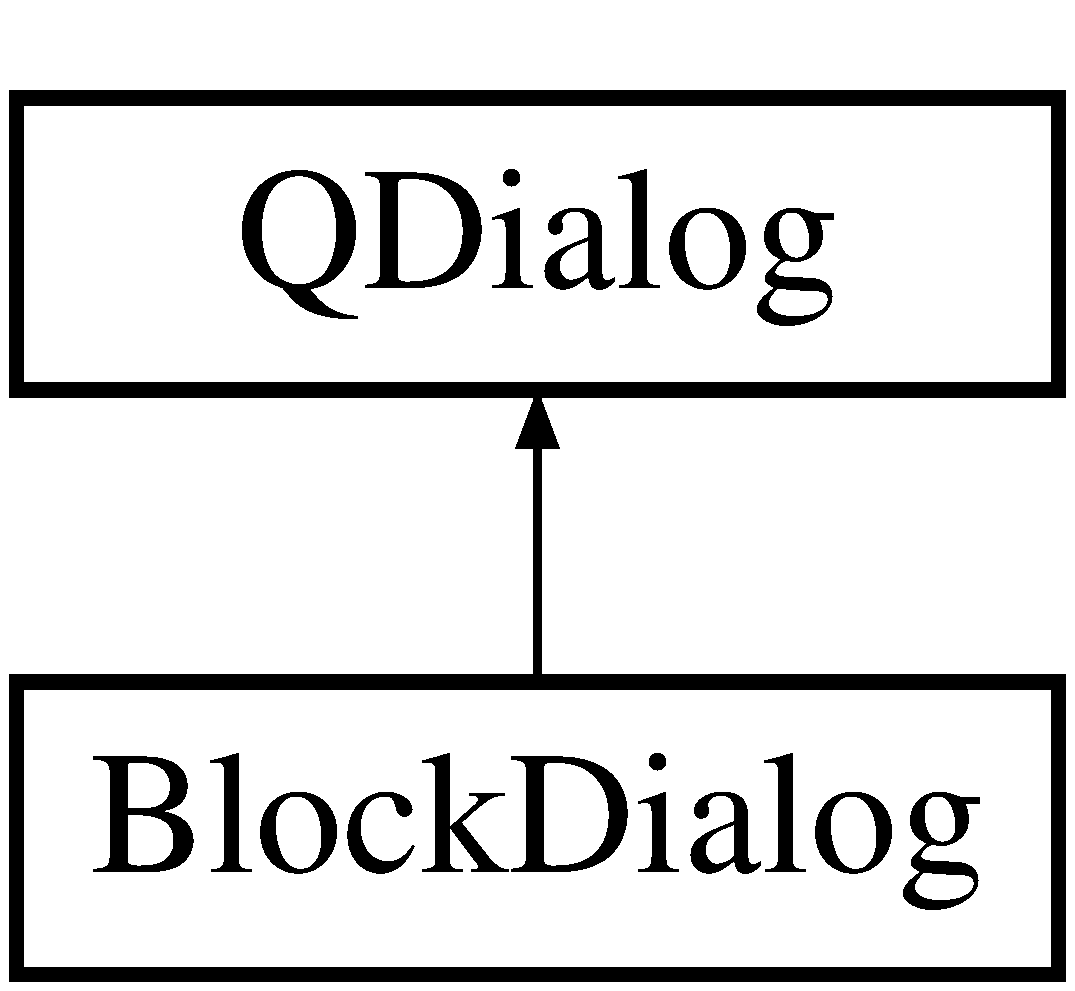
\includegraphics[height=2.000000cm]{classBlockDialog}
\end{center}
\end{figure}
\subsection*{Public Member Functions}
\begin{DoxyCompactItemize}
\item 
\hyperlink{classBlockDialog_ab73c3fae34eb587bee67c0b67974c97e}{Block\+Dialog} (Q\+Widget $\ast$parent=0)
\item 
\hyperlink{classBlockDialog_a7a524e7d75f6b0c0addb855de52d713f}{$\sim$\+Block\+Dialog} ()
\end{DoxyCompactItemize}
\subsection*{Private Slots}
\begin{DoxyCompactItemize}
\item 
void \hyperlink{classBlockDialog_ad8f20cab9c17a9a03d846a10215c55c5}{on\+\_\+\+A\+D\+D\+\_\+clicked} ()
\item 
void \hyperlink{classBlockDialog_af9974e5eed00d8ed6541207152559639}{on\+\_\+\+S\+U\+B\+\_\+clicked} ()
\item 
void \hyperlink{classBlockDialog_a8d9ff3eb620ffcf02a184b7a5ca535ce}{on\+\_\+\+M\+U\+L\+\_\+clicked} ()
\item 
void \hyperlink{classBlockDialog_a01cf45f68a5b5b688916be2a8d78e7eb}{on\+\_\+\+D\+I\+V\+\_\+clicked} ()
\item 
void \hyperlink{classBlockDialog_aaa26399a715ce36bf46f9c4a7a3b834a}{on\+\_\+\+I\+N\+\_\+clicked} ()
\item 
void \hyperlink{classBlockDialog_ab5afbbd67eb4c1ee11191cad1da29630}{on\+\_\+\+O\+U\+T\+\_\+clicked} ()
\item 
void \hyperlink{classBlockDialog_a5e445ed193d3f7e2eba29e192f038221}{on\+\_\+\+Apply\+\_\+clicked} ()
\item 
void \hyperlink{classBlockDialog_a9c009de0d86bff7a265f3db598e204fc}{on\+\_\+horizontal\+Slider\+\_\+slider\+Moved} (int \hyperlink{classBlockDialog_ad0c5a84d24461a66fc604159306cd65c}{value})
\item 
void \hyperlink{classBlockDialog_a875bd7ee646be1c30b90f09d3666b4b1}{on\+\_\+\+Cancel\+\_\+clicked} ()
\item 
void \hyperlink{classBlockDialog_aadce9fabc644d0d73f36ddc3749c9975}{on\+\_\+line\+Edit\+\_\+text\+Changed} (const Q\+String \&arg1)
\end{DoxyCompactItemize}
\subsection*{Private Attributes}
\begin{DoxyCompactItemize}
\item 
E\+Block \hyperlink{classBlockDialog_a369bf9158760dcf32d7c98d7f4c3fd24}{selected}
\item 
double \hyperlink{classBlockDialog_ad0c5a84d24461a66fc604159306cd65c}{value}
\item 
int \hyperlink{classBlockDialog_a5d3f519ebe7794146a1f24607ab3066a}{port\+Count} = 2
\item 
Ui\+::\+Block\+Dialog $\ast$ \hyperlink{classBlockDialog_ad8e54f70336f615f84a19cf59b4bb420}{ui}
\end{DoxyCompactItemize}


\subsection{Constructor \& Destructor Documentation}
\mbox{\Hypertarget{classBlockDialog_ab73c3fae34eb587bee67c0b67974c97e}\label{classBlockDialog_ab73c3fae34eb587bee67c0b67974c97e}} 
\index{Block\+Dialog@{Block\+Dialog}!Block\+Dialog@{Block\+Dialog}}
\index{Block\+Dialog@{Block\+Dialog}!Block\+Dialog@{Block\+Dialog}}
\subsubsection{\texorpdfstring{Block\+Dialog()}{BlockDialog()}}
{\footnotesize\ttfamily Block\+Dialog\+::\+Block\+Dialog (\begin{DoxyParamCaption}\item[{Q\+Widget $\ast$}]{parent = {\ttfamily 0} }\end{DoxyParamCaption})\hspace{0.3cm}{\ttfamily [explicit]}}

The explicit constructor to create new instance.


\begin{DoxyParams}{Parameters}
{\em parent} & parameter where it will be draw. \\
\hline
\end{DoxyParams}
\mbox{\Hypertarget{classBlockDialog_a7a524e7d75f6b0c0addb855de52d713f}\label{classBlockDialog_a7a524e7d75f6b0c0addb855de52d713f}} 
\index{Block\+Dialog@{Block\+Dialog}!````~Block\+Dialog@{$\sim$\+Block\+Dialog}}
\index{````~Block\+Dialog@{$\sim$\+Block\+Dialog}!Block\+Dialog@{Block\+Dialog}}
\subsubsection{\texorpdfstring{$\sim$\+Block\+Dialog()}{~BlockDialog()}}
{\footnotesize\ttfamily Block\+Dialog\+::$\sim$\+Block\+Dialog (\begin{DoxyParamCaption}{ }\end{DoxyParamCaption})}

Destructor that clears window and destroy all objects on it. 

\subsection{Member Function Documentation}
\mbox{\Hypertarget{classBlockDialog_ad8f20cab9c17a9a03d846a10215c55c5}\label{classBlockDialog_ad8f20cab9c17a9a03d846a10215c55c5}} 
\index{Block\+Dialog@{Block\+Dialog}!on\+\_\+\+A\+D\+D\+\_\+clicked@{on\+\_\+\+A\+D\+D\+\_\+clicked}}
\index{on\+\_\+\+A\+D\+D\+\_\+clicked@{on\+\_\+\+A\+D\+D\+\_\+clicked}!Block\+Dialog@{Block\+Dialog}}
\subsubsection{\texorpdfstring{on\+\_\+\+A\+D\+D\+\_\+clicked}{on\_ADD\_clicked}}
{\footnotesize\ttfamily void Block\+Dialog\+::on\+\_\+\+A\+D\+D\+\_\+clicked (\begin{DoxyParamCaption}{ }\end{DoxyParamCaption})\hspace{0.3cm}{\ttfamily [private]}, {\ttfamily [slot]}}

Event calls by click on add button. It sets selected operation. \mbox{\Hypertarget{classBlockDialog_a5e445ed193d3f7e2eba29e192f038221}\label{classBlockDialog_a5e445ed193d3f7e2eba29e192f038221}} 
\index{Block\+Dialog@{Block\+Dialog}!on\+\_\+\+Apply\+\_\+clicked@{on\+\_\+\+Apply\+\_\+clicked}}
\index{on\+\_\+\+Apply\+\_\+clicked@{on\+\_\+\+Apply\+\_\+clicked}!Block\+Dialog@{Block\+Dialog}}
\subsubsection{\texorpdfstring{on\+\_\+\+Apply\+\_\+clicked}{on\_Apply\_clicked}}
{\footnotesize\ttfamily void Block\+Dialog\+::on\+\_\+\+Apply\+\_\+clicked (\begin{DoxyParamCaption}{ }\end{DoxyParamCaption})\hspace{0.3cm}{\ttfamily [private]}, {\ttfamily [slot]}}

Event calls by click on Apply button. Creates new block by selected type and closes the popup window. \mbox{\Hypertarget{classBlockDialog_a875bd7ee646be1c30b90f09d3666b4b1}\label{classBlockDialog_a875bd7ee646be1c30b90f09d3666b4b1}} 
\index{Block\+Dialog@{Block\+Dialog}!on\+\_\+\+Cancel\+\_\+clicked@{on\+\_\+\+Cancel\+\_\+clicked}}
\index{on\+\_\+\+Cancel\+\_\+clicked@{on\+\_\+\+Cancel\+\_\+clicked}!Block\+Dialog@{Block\+Dialog}}
\subsubsection{\texorpdfstring{on\+\_\+\+Cancel\+\_\+clicked}{on\_Cancel\_clicked}}
{\footnotesize\ttfamily void Block\+Dialog\+::on\+\_\+\+Cancel\+\_\+clicked (\begin{DoxyParamCaption}{ }\end{DoxyParamCaption})\hspace{0.3cm}{\ttfamily [private]}, {\ttfamily [slot]}}

Event calls by click on Cancel button. It closes the window it its not needed. \mbox{\Hypertarget{classBlockDialog_a01cf45f68a5b5b688916be2a8d78e7eb}\label{classBlockDialog_a01cf45f68a5b5b688916be2a8d78e7eb}} 
\index{Block\+Dialog@{Block\+Dialog}!on\+\_\+\+D\+I\+V\+\_\+clicked@{on\+\_\+\+D\+I\+V\+\_\+clicked}}
\index{on\+\_\+\+D\+I\+V\+\_\+clicked@{on\+\_\+\+D\+I\+V\+\_\+clicked}!Block\+Dialog@{Block\+Dialog}}
\subsubsection{\texorpdfstring{on\+\_\+\+D\+I\+V\+\_\+clicked}{on\_DIV\_clicked}}
{\footnotesize\ttfamily void Block\+Dialog\+::on\+\_\+\+D\+I\+V\+\_\+clicked (\begin{DoxyParamCaption}{ }\end{DoxyParamCaption})\hspace{0.3cm}{\ttfamily [private]}, {\ttfamily [slot]}}

Event calls by click on D\+IV button. It sets selected operation. \mbox{\Hypertarget{classBlockDialog_a9c009de0d86bff7a265f3db598e204fc}\label{classBlockDialog_a9c009de0d86bff7a265f3db598e204fc}} 
\index{Block\+Dialog@{Block\+Dialog}!on\+\_\+horizontal\+Slider\+\_\+slider\+Moved@{on\+\_\+horizontal\+Slider\+\_\+slider\+Moved}}
\index{on\+\_\+horizontal\+Slider\+\_\+slider\+Moved@{on\+\_\+horizontal\+Slider\+\_\+slider\+Moved}!Block\+Dialog@{Block\+Dialog}}
\subsubsection{\texorpdfstring{on\+\_\+horizontal\+Slider\+\_\+slider\+Moved}{on\_horizontalSlider\_sliderMoved}}
{\footnotesize\ttfamily void Block\+Dialog\+::on\+\_\+horizontal\+Slider\+\_\+slider\+Moved (\begin{DoxyParamCaption}\item[{int}]{value }\end{DoxyParamCaption})\hspace{0.3cm}{\ttfamily [private]}, {\ttfamily [slot]}}

Event calls by moving slider on window. Slider sets number of input ports on block. Default value of slider is 2 and its hidden while IN block is selected, because IN block doesnt have any input ports.


\begin{DoxyParams}{Parameters}
{\em value} & returns value that slider have. \\
\hline
\end{DoxyParams}
\mbox{\Hypertarget{classBlockDialog_aaa26399a715ce36bf46f9c4a7a3b834a}\label{classBlockDialog_aaa26399a715ce36bf46f9c4a7a3b834a}} 
\index{Block\+Dialog@{Block\+Dialog}!on\+\_\+\+I\+N\+\_\+clicked@{on\+\_\+\+I\+N\+\_\+clicked}}
\index{on\+\_\+\+I\+N\+\_\+clicked@{on\+\_\+\+I\+N\+\_\+clicked}!Block\+Dialog@{Block\+Dialog}}
\subsubsection{\texorpdfstring{on\+\_\+\+I\+N\+\_\+clicked}{on\_IN\_clicked}}
{\footnotesize\ttfamily void Block\+Dialog\+::on\+\_\+\+I\+N\+\_\+clicked (\begin{DoxyParamCaption}{ }\end{DoxyParamCaption})\hspace{0.3cm}{\ttfamily [private]}, {\ttfamily [slot]}}

Event calls by click on IN button. It sets selected operation. \mbox{\Hypertarget{classBlockDialog_aadce9fabc644d0d73f36ddc3749c9975}\label{classBlockDialog_aadce9fabc644d0d73f36ddc3749c9975}} 
\index{Block\+Dialog@{Block\+Dialog}!on\+\_\+line\+Edit\+\_\+text\+Changed@{on\+\_\+line\+Edit\+\_\+text\+Changed}}
\index{on\+\_\+line\+Edit\+\_\+text\+Changed@{on\+\_\+line\+Edit\+\_\+text\+Changed}!Block\+Dialog@{Block\+Dialog}}
\subsubsection{\texorpdfstring{on\+\_\+line\+Edit\+\_\+text\+Changed}{on\_lineEdit\_textChanged}}
{\footnotesize\ttfamily void Block\+Dialog\+::on\+\_\+line\+Edit\+\_\+text\+Changed (\begin{DoxyParamCaption}\item[{const Q\+String \&}]{arg1 }\end{DoxyParamCaption})\hspace{0.3cm}{\ttfamily [private]}, {\ttfamily [slot]}}

Event calls by writing text into textbox. The text should be only number. The textbox is showed if the IN block is selected.


\begin{DoxyParams}{Parameters}
{\em arg1} & returns value that IN block have to have. \\
\hline
\end{DoxyParams}
\mbox{\Hypertarget{classBlockDialog_a8d9ff3eb620ffcf02a184b7a5ca535ce}\label{classBlockDialog_a8d9ff3eb620ffcf02a184b7a5ca535ce}} 
\index{Block\+Dialog@{Block\+Dialog}!on\+\_\+\+M\+U\+L\+\_\+clicked@{on\+\_\+\+M\+U\+L\+\_\+clicked}}
\index{on\+\_\+\+M\+U\+L\+\_\+clicked@{on\+\_\+\+M\+U\+L\+\_\+clicked}!Block\+Dialog@{Block\+Dialog}}
\subsubsection{\texorpdfstring{on\+\_\+\+M\+U\+L\+\_\+clicked}{on\_MUL\_clicked}}
{\footnotesize\ttfamily void Block\+Dialog\+::on\+\_\+\+M\+U\+L\+\_\+clicked (\begin{DoxyParamCaption}{ }\end{DoxyParamCaption})\hspace{0.3cm}{\ttfamily [private]}, {\ttfamily [slot]}}

Event calls by click on M\+UL button. It sets selected operation. \mbox{\Hypertarget{classBlockDialog_ab5afbbd67eb4c1ee11191cad1da29630}\label{classBlockDialog_ab5afbbd67eb4c1ee11191cad1da29630}} 
\index{Block\+Dialog@{Block\+Dialog}!on\+\_\+\+O\+U\+T\+\_\+clicked@{on\+\_\+\+O\+U\+T\+\_\+clicked}}
\index{on\+\_\+\+O\+U\+T\+\_\+clicked@{on\+\_\+\+O\+U\+T\+\_\+clicked}!Block\+Dialog@{Block\+Dialog}}
\subsubsection{\texorpdfstring{on\+\_\+\+O\+U\+T\+\_\+clicked}{on\_OUT\_clicked}}
{\footnotesize\ttfamily void Block\+Dialog\+::on\+\_\+\+O\+U\+T\+\_\+clicked (\begin{DoxyParamCaption}{ }\end{DoxyParamCaption})\hspace{0.3cm}{\ttfamily [private]}, {\ttfamily [slot]}}

Event calls by click on O\+UT button. It sets selected operation. \mbox{\Hypertarget{classBlockDialog_af9974e5eed00d8ed6541207152559639}\label{classBlockDialog_af9974e5eed00d8ed6541207152559639}} 
\index{Block\+Dialog@{Block\+Dialog}!on\+\_\+\+S\+U\+B\+\_\+clicked@{on\+\_\+\+S\+U\+B\+\_\+clicked}}
\index{on\+\_\+\+S\+U\+B\+\_\+clicked@{on\+\_\+\+S\+U\+B\+\_\+clicked}!Block\+Dialog@{Block\+Dialog}}
\subsubsection{\texorpdfstring{on\+\_\+\+S\+U\+B\+\_\+clicked}{on\_SUB\_clicked}}
{\footnotesize\ttfamily void Block\+Dialog\+::on\+\_\+\+S\+U\+B\+\_\+clicked (\begin{DoxyParamCaption}{ }\end{DoxyParamCaption})\hspace{0.3cm}{\ttfamily [private]}, {\ttfamily [slot]}}

Event calls by click on S\+UB button. It sets selected operation. 

\subsection{Member Data Documentation}
\mbox{\Hypertarget{classBlockDialog_a5d3f519ebe7794146a1f24607ab3066a}\label{classBlockDialog_a5d3f519ebe7794146a1f24607ab3066a}} 
\index{Block\+Dialog@{Block\+Dialog}!port\+Count@{port\+Count}}
\index{port\+Count@{port\+Count}!Block\+Dialog@{Block\+Dialog}}
\subsubsection{\texorpdfstring{port\+Count}{portCount}}
{\footnotesize\ttfamily int Block\+Dialog\+::port\+Count = 2\hspace{0.3cm}{\ttfamily [private]}}

Default value of ports it sets the slider. \mbox{\Hypertarget{classBlockDialog_a369bf9158760dcf32d7c98d7f4c3fd24}\label{classBlockDialog_a369bf9158760dcf32d7c98d7f4c3fd24}} 
\index{Block\+Dialog@{Block\+Dialog}!selected@{selected}}
\index{selected@{selected}!Block\+Dialog@{Block\+Dialog}}
\subsubsection{\texorpdfstring{selected}{selected}}
{\footnotesize\ttfamily E\+Block Block\+Dialog\+::selected\hspace{0.3cm}{\ttfamily [private]}}

Type of new block that buttons sets. \mbox{\Hypertarget{classBlockDialog_ad8e54f70336f615f84a19cf59b4bb420}\label{classBlockDialog_ad8e54f70336f615f84a19cf59b4bb420}} 
\index{Block\+Dialog@{Block\+Dialog}!ui@{ui}}
\index{ui@{ui}!Block\+Dialog@{Block\+Dialog}}
\subsubsection{\texorpdfstring{ui}{ui}}
{\footnotesize\ttfamily Ui\+::\+Block\+Dialog$\ast$ Block\+Dialog\+::ui\hspace{0.3cm}{\ttfamily [private]}}

Ui variable that shows me available components on panel. \mbox{\Hypertarget{classBlockDialog_ad0c5a84d24461a66fc604159306cd65c}\label{classBlockDialog_ad0c5a84d24461a66fc604159306cd65c}} 
\index{Block\+Dialog@{Block\+Dialog}!value@{value}}
\index{value@{value}!Block\+Dialog@{Block\+Dialog}}
\subsubsection{\texorpdfstring{value}{value}}
{\footnotesize\ttfamily double Block\+Dialog\+::value\hspace{0.3cm}{\ttfamily [private]}}

Value that IN block have on his out port. 

The documentation for this class was generated from the following files\+:\begin{DoxyCompactItemize}
\item 
blockdialog.\+h\item 
blockdialog.\+cpp\end{DoxyCompactItemize}

\hypertarget{classDrawableObject}{}\section{Drawable\+Object Class Reference}
\label{classDrawableObject}\index{Drawable\+Object@{Drawable\+Object}}
Inheritance diagram for Drawable\+Object\+:\begin{figure}[H]
\begin{center}
\leavevmode
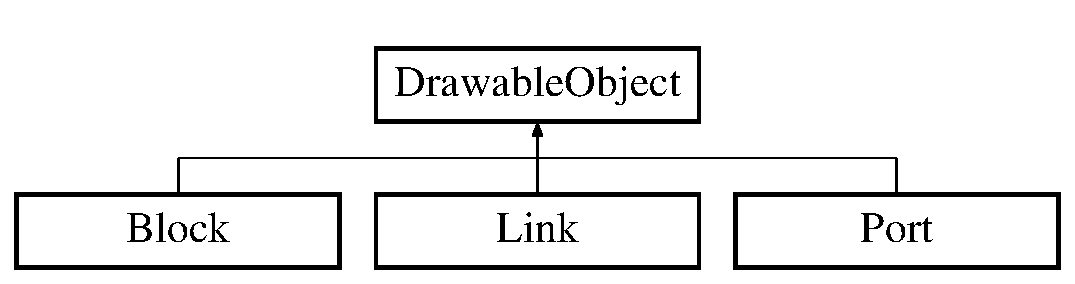
\includegraphics[height=2.000000cm]{classDrawableObject}
\end{center}
\end{figure}
\subsection*{Public Member Functions}
\begin{DoxyCompactItemize}
\item 
\mbox{\Hypertarget{classDrawableObject_a107d5c6f1ec88d09582610c2612630c9}\label{classDrawableObject_a107d5c6f1ec88d09582610c2612630c9}} 
virtual void {\bfseries Draw} (Q\+Painter $\ast$)
\end{DoxyCompactItemize}


The documentation for this class was generated from the following files\+:\begin{DoxyCompactItemize}
\item 
drawableobject.\+h\item 
drawableobject.\+cpp\end{DoxyCompactItemize}

\hypertarget{classLink}{}\section{Link Class Reference}
\label{classLink}\index{Link@{Link}}
Inheritance diagram for Link\+:\begin{figure}[H]
\begin{center}
\leavevmode
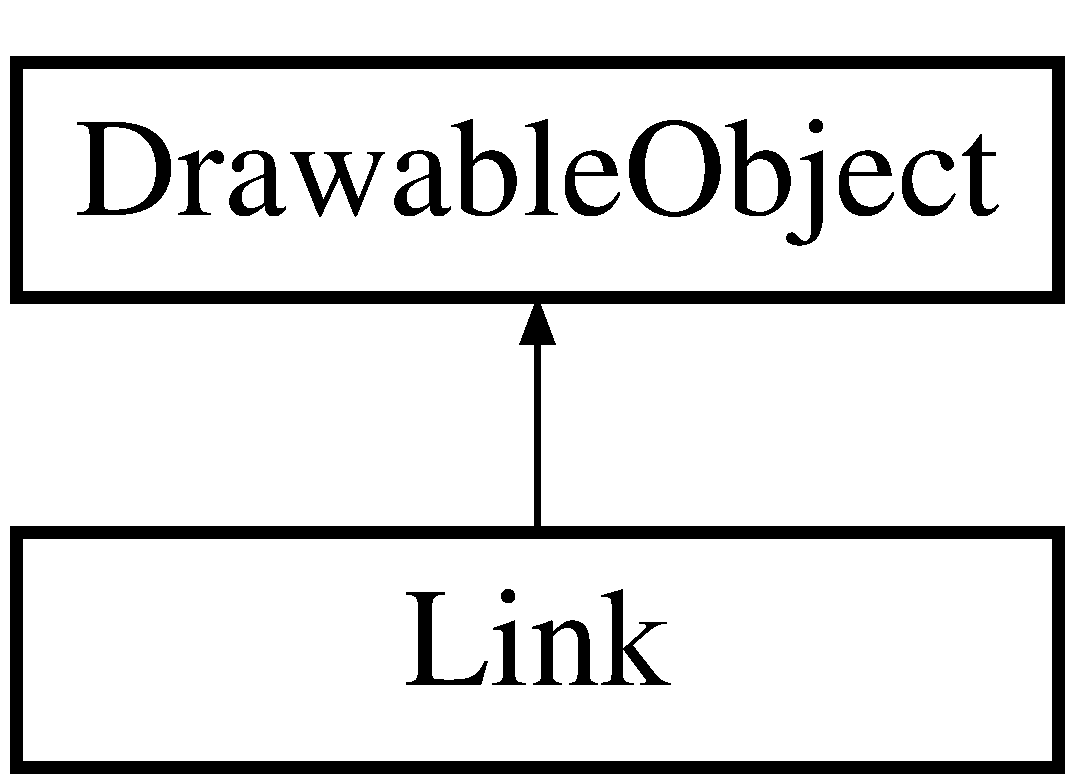
\includegraphics[height=2.000000cm]{classLink}
\end{center}
\end{figure}
\subsection*{Public Member Functions}
\begin{DoxyCompactItemize}
\item 
\mbox{\Hypertarget{classLink_a2db8894bce4b94c941fe973f46d63600}\label{classLink_a2db8894bce4b94c941fe973f46d63600}} 
{\bfseries Link} (const \hyperlink{classLink}{Link} \&)
\item 
\mbox{\Hypertarget{classLink_a4d958d9cfbb214cd244f997958c5f1ad}\label{classLink_a4d958d9cfbb214cd244f997958c5f1ad}} 
{\bfseries Link} (\hyperlink{classPort}{Port} $\ast$, \hyperlink{classPort}{Port} $\ast$)
\item 
\mbox{\Hypertarget{classLink_abd0c01cc4f2327c0ae4fd8ab6af07653}\label{classLink_abd0c01cc4f2327c0ae4fd8ab6af07653}} 
\hyperlink{classPort}{Port} $\ast$ {\bfseries get\+In\+Port} ()
\item 
\mbox{\Hypertarget{classLink_a6b574d3c11ee9bba28509e5d85acaa94}\label{classLink_a6b574d3c11ee9bba28509e5d85acaa94}} 
\hyperlink{classPort}{Port} $\ast$ {\bfseries get\+Out\+Port} ()
\item 
\mbox{\Hypertarget{classLink_a2689e0202d4a1d1b39588abd25241417}\label{classLink_a2689e0202d4a1d1b39588abd25241417}} 
void {\bfseries set\+In\+Port} (\hyperlink{classPort}{Port} $\ast$)
\item 
\mbox{\Hypertarget{classLink_aa04660e88b32ea60c0209482a6bc68c1}\label{classLink_aa04660e88b32ea60c0209482a6bc68c1}} 
void {\bfseries set\+Out\+Port} (\hyperlink{classPort}{Port} $\ast$)
\item 
\mbox{\Hypertarget{classLink_a83ac4b54c4b0a240701821c2c195364e}\label{classLink_a83ac4b54c4b0a240701821c2c195364e}} 
Q\+Line $\ast$ {\bfseries get\+Line} ()
\item 
\mbox{\Hypertarget{classLink_a0e08eb4518bc88e7b74e6581badd91fd}\label{classLink_a0e08eb4518bc88e7b74e6581badd91fd}} 
bool {\bfseries Is\+Cycled} ()
\item 
\mbox{\Hypertarget{classLink_ac9f06bd0dd2272222b62102a94cf6607}\label{classLink_ac9f06bd0dd2272222b62102a94cf6607}} 
void {\bfseries Set\+Cycled} ()
\item 
\mbox{\Hypertarget{classLink_a41ec810a02d72f2aa6e2c049075dd026}\label{classLink_a41ec810a02d72f2aa6e2c049075dd026}} 
void {\bfseries Un\+Set\+Cycled} ()
\item 
\mbox{\Hypertarget{classLink_ab150ec2cc71a241be7e3abd40837f369}\label{classLink_ab150ec2cc71a241be7e3abd40837f369}} 
virtual void {\bfseries Draw} (Q\+Painter $\ast$) override
\end{DoxyCompactItemize}
\subsection*{Static Public Member Functions}
\begin{DoxyCompactItemize}
\item 
\mbox{\Hypertarget{classLink_a2b815f1d35a5588416190e7ea0a11b63}\label{classLink_a2b815f1d35a5588416190e7ea0a11b63}} 
static bool {\bfseries Is\+Point\+On\+Line} (Q\+Line $\ast$line, \hyperlink{classPoint2D}{Point2D} $\ast$point)
\end{DoxyCompactItemize}
\subsection*{Private Attributes}
\begin{DoxyCompactItemize}
\item 
\mbox{\Hypertarget{classLink_a6e935a336f4a03071fcc2b592276c4ca}\label{classLink_a6e935a336f4a03071fcc2b592276c4ca}} 
\hyperlink{classPort}{Port} $\ast$ {\bfseries in\+Port} = nullptr
\item 
\mbox{\Hypertarget{classLink_a0e326445a40f370fbaec9b1bbfd3fc2d}\label{classLink_a0e326445a40f370fbaec9b1bbfd3fc2d}} 
\hyperlink{classPort}{Port} $\ast$ {\bfseries out\+Port} = nullptr
\item 
\mbox{\Hypertarget{classLink_af181aac9843b389800939c294c01d4ac}\label{classLink_af181aac9843b389800939c294c01d4ac}} 
Q\+Line $\ast$ {\bfseries line} = nullptr
\item 
\mbox{\Hypertarget{classLink_a70e3252b06be7f81d6345ad1197dc18c}\label{classLink_a70e3252b06be7f81d6345ad1197dc18c}} 
bool {\bfseries is\+Cycled}
\end{DoxyCompactItemize}


The documentation for this class was generated from the following files\+:\begin{DoxyCompactItemize}
\item 
link.\+h\item 
link.\+cpp\end{DoxyCompactItemize}

\hypertarget{classLoadManager}{}\section{Load\+Manager Class Reference}
\label{classLoadManager}\index{Load\+Manager@{Load\+Manager}}
\subsection*{Static Public Member Functions}
\begin{DoxyCompactItemize}
\item 
\mbox{\Hypertarget{classLoadManager_a3f96fe7100a7b76fd63e8500b89bd84c}\label{classLoadManager_a3f96fe7100a7b76fd63e8500b89bd84c}} 
static bool {\bfseries save\+Scene} ()
\item 
\mbox{\Hypertarget{classLoadManager_a2836efb2f4a790d0c86d10de9ff9a1f2}\label{classLoadManager_a2836efb2f4a790d0c86d10de9ff9a1f2}} 
static void {\bfseries load\+Scene} ()
\end{DoxyCompactItemize}


The documentation for this class was generated from the following files\+:\begin{DoxyCompactItemize}
\item 
loadmanager.\+h\item 
loadmanager.\+cpp\end{DoxyCompactItemize}

\hypertarget{classMyRect}{}\section{My\+Rect Class Reference}
\label{classMyRect}\index{My\+Rect@{My\+Rect}}
Inheritance diagram for My\+Rect\+:\begin{figure}[H]
\begin{center}
\leavevmode
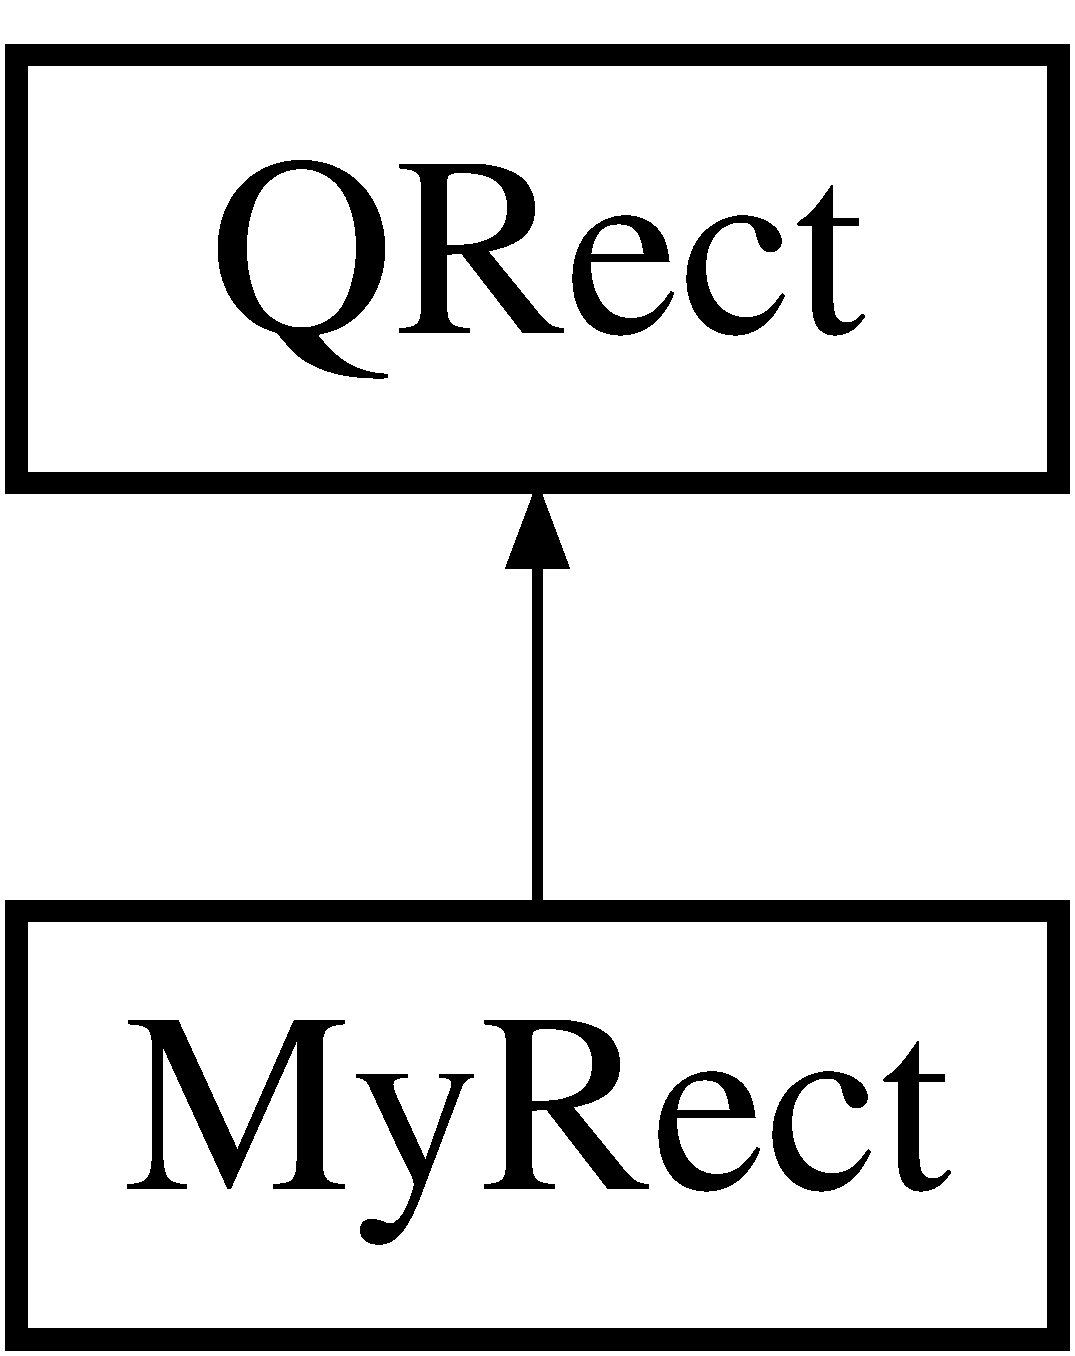
\includegraphics[height=2.000000cm]{classMyRect}
\end{center}
\end{figure}
\subsection*{Public Member Functions}
\begin{DoxyCompactItemize}
\item 
\mbox{\Hypertarget{classMyRect_aa52fa58a67a98f01b5e63e7788205728}\label{classMyRect_aa52fa58a67a98f01b5e63e7788205728}} 
{\bfseries My\+Rect} (const \hyperlink{classMyRect}{My\+Rect} \&)
\item 
\mbox{\Hypertarget{classMyRect_adae6a6df7e9da17eea5dd74887fc9f99}\label{classMyRect_adae6a6df7e9da17eea5dd74887fc9f99}} 
{\bfseries My\+Rect} (\hyperlink{classPoint2D}{Point2D}, \hyperlink{classPoint2D}{Point2D})
\item 
\mbox{\Hypertarget{classMyRect_a3266e6b3de8ddbbb036f94df96f30925}\label{classMyRect_a3266e6b3de8ddbbb036f94df96f30925}} 
{\bfseries My\+Rect} (double, double, \hyperlink{classPoint2D}{Point2D})
\item 
\mbox{\Hypertarget{classMyRect_a2fc305015dd715acfa29309c16affc06}\label{classMyRect_a2fc305015dd715acfa29309c16affc06}} 
{\bfseries My\+Rect} (\hyperlink{classPoint2D}{Point2D}, double, double)
\item 
\mbox{\Hypertarget{classMyRect_ad9bcb336c9fb635e0a33ec3e6dfe6942}\label{classMyRect_ad9bcb336c9fb635e0a33ec3e6dfe6942}} 
{\bfseries My\+Rect} (double, double, double, double)
\item 
\mbox{\Hypertarget{classMyRect_a1949f02801a73e06cdc7bb31245975d4}\label{classMyRect_a1949f02801a73e06cdc7bb31245975d4}} 
bool {\bfseries contains} (\hyperlink{classPoint2D}{Point2D} $\ast$)
\item 
\mbox{\Hypertarget{classMyRect_af6397c8b42b9956f6962e8ae92466058}\label{classMyRect_af6397c8b42b9956f6962e8ae92466058}} 
bool {\bfseries intersect} (\hyperlink{classMyRect}{My\+Rect} $\ast$)
\item 
\mbox{\Hypertarget{classMyRect_a0b62fe4edec3e3fe51eb1d26daf373b2}\label{classMyRect_a0b62fe4edec3e3fe51eb1d26daf373b2}} 
double {\bfseries X\+Min} ()
\item 
\mbox{\Hypertarget{classMyRect_a8d03cd598ce637cc3e5129e57fae2f1f}\label{classMyRect_a8d03cd598ce637cc3e5129e57fae2f1f}} 
double {\bfseries X\+Max} ()
\item 
\mbox{\Hypertarget{classMyRect_a92c2a3eb0f31fde949acc622d1482a66}\label{classMyRect_a92c2a3eb0f31fde949acc622d1482a66}} 
double {\bfseries Y\+Min} ()
\item 
\mbox{\Hypertarget{classMyRect_a086e41548aa99301b00fb0b53285cf0e}\label{classMyRect_a086e41548aa99301b00fb0b53285cf0e}} 
double {\bfseries Y\+Max} ()
\item 
\mbox{\Hypertarget{classMyRect_a16fcae840ff7542836e2256713c42803}\label{classMyRect_a16fcae840ff7542836e2256713c42803}} 
\hyperlink{classPoint2D}{Point2D} $\ast$ {\bfseries Position} ()
\item 
\mbox{\Hypertarget{classMyRect_ad9bc8a8c51f3c99bdcb0ea417757a086}\label{classMyRect_ad9bc8a8c51f3c99bdcb0ea417757a086}} 
\hyperlink{classPoint2D}{Point2D} $\ast$ {\bfseries Size} ()
\item 
\mbox{\Hypertarget{classMyRect_a54af9ff8c6856ee11ea43b5499707877}\label{classMyRect_a54af9ff8c6856ee11ea43b5499707877}} 
\hyperlink{classPoint2D}{Point2D} $\ast$ {\bfseries Center} ()
\item 
\mbox{\Hypertarget{classMyRect_a87d65ecd22add421fc3a2a9ac777ce91}\label{classMyRect_a87d65ecd22add421fc3a2a9ac777ce91}} 
virtual void {\bfseries mouse\+Clicked\+Event} (Q\+Mouse\+Event $\ast$e)
\end{DoxyCompactItemize}
\subsection*{Friends}
\begin{DoxyCompactItemize}
\item 
\mbox{\Hypertarget{classMyRect_a0776fa667a382b15220104e62f6d4f7b}\label{classMyRect_a0776fa667a382b15220104e62f6d4f7b}} 
std\+::istream \& {\bfseries operator$>$$>$} (std\+::istream \&is, \hyperlink{classMyRect}{My\+Rect} \&rect)
\item 
\mbox{\Hypertarget{classMyRect_a7d9295e04322b6022fabd8cbff944c3e}\label{classMyRect_a7d9295e04322b6022fabd8cbff944c3e}} 
std\+::ostream \& {\bfseries operator$<$$<$} (std\+::ostream \&os, \hyperlink{classMyRect}{My\+Rect} \&rect)
\end{DoxyCompactItemize}


The documentation for this class was generated from the following files\+:\begin{DoxyCompactItemize}
\item 
myrect.\+h\item 
myrect.\+cpp\end{DoxyCompactItemize}

\hypertarget{classPoint2D}{}\section{Point2D Class Reference}
\label{classPoint2D}\index{Point2D@{Point2D}}
\subsection*{Public Member Functions}
\begin{DoxyCompactItemize}
\item 
\mbox{\Hypertarget{classPoint2D_a0e3ee506aac9ae6461bdf6083c7596b0}\label{classPoint2D_a0e3ee506aac9ae6461bdf6083c7596b0}} 
{\bfseries Point2D} (double, double)
\item 
\mbox{\Hypertarget{classPoint2D_a6853dff081e82d0349b349cc2362b360}\label{classPoint2D_a6853dff081e82d0349b349cc2362b360}} 
\hyperlink{classPoint2D}{Point2D} {\bfseries sub} (\hyperlink{classPoint2D}{Point2D})
\item 
\mbox{\Hypertarget{classPoint2D_a26f33af7a25257f0e87ddbeeb65e9fb9}\label{classPoint2D_a26f33af7a25257f0e87ddbeeb65e9fb9}} 
\hyperlink{classPoint2D}{Point2D} {\bfseries add} (\hyperlink{classPoint2D}{Point2D})
\end{DoxyCompactItemize}
\subsection*{Static Public Member Functions}
\begin{DoxyCompactItemize}
\item 
\mbox{\Hypertarget{classPoint2D_ad5491be33bca3403d4e1d20e42b30750}\label{classPoint2D_ad5491be33bca3403d4e1d20e42b30750}} 
static double {\bfseries distance} (\hyperlink{classPoint2D}{Point2D}, \hyperlink{classPoint2D}{Point2D})
\item 
\mbox{\Hypertarget{classPoint2D_ad823958e5f2041fa3b4e433b3ce17b2f}\label{classPoint2D_ad823958e5f2041fa3b4e433b3ce17b2f}} 
static \hyperlink{classPoint2D}{Point2D} $\ast$ {\bfseries vector} (\hyperlink{classPoint2D}{Point2D} $\ast$, \hyperlink{classPoint2D}{Point2D} $\ast$)
\end{DoxyCompactItemize}
\subsection*{Public Attributes}
\begin{DoxyCompactItemize}
\item 
\mbox{\Hypertarget{classPoint2D_a18681fb0a8389c0c501d6e38f90cc1b5}\label{classPoint2D_a18681fb0a8389c0c501d6e38f90cc1b5}} 
double {\bfseries X}
\item 
\mbox{\Hypertarget{classPoint2D_ab2b22ea52c6db3697fd8ce4827103654}\label{classPoint2D_ab2b22ea52c6db3697fd8ce4827103654}} 
double {\bfseries Y}
\end{DoxyCompactItemize}
\subsection*{Friends}
\begin{DoxyCompactItemize}
\item 
\mbox{\Hypertarget{classPoint2D_a09b15e84ab259e853b28c2eb56b10713}\label{classPoint2D_a09b15e84ab259e853b28c2eb56b10713}} 
std\+::ostream \& {\bfseries operator$<$$<$} (std\+::ostream \&os, \hyperlink{classPoint2D}{Point2D} \&point)
\end{DoxyCompactItemize}


The documentation for this class was generated from the following files\+:\begin{DoxyCompactItemize}
\item 
point2d.\+h\item 
point2d.\+cpp\end{DoxyCompactItemize}

\hypertarget{classPort}{}\section{Port Class Reference}
\label{classPort}\index{Port@{Port}}
Inheritance diagram for Port\+:\begin{figure}[H]
\begin{center}
\leavevmode
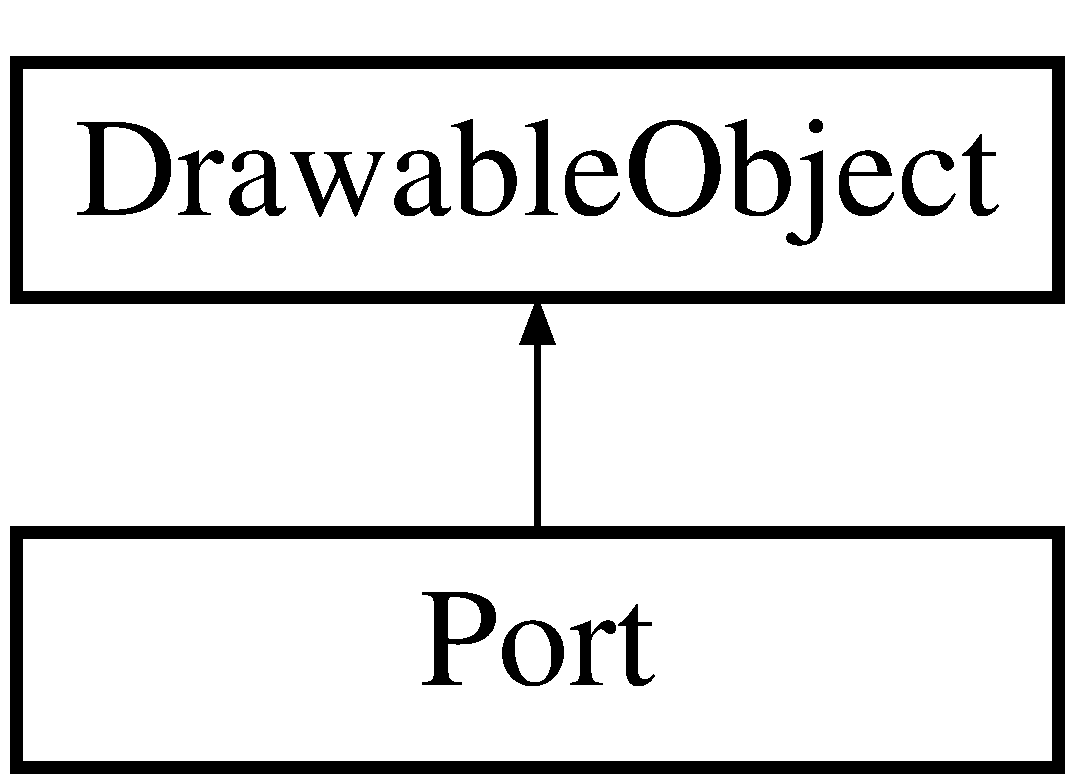
\includegraphics[height=2.000000cm]{classPort}
\end{center}
\end{figure}
\subsection*{Public Member Functions}
\begin{DoxyCompactItemize}
\item 
\mbox{\Hypertarget{classPort_a2771ea55321da837962228239ad197f4}\label{classPort_a2771ea55321da837962228239ad197f4}} 
std\+::vector$<$ \hyperlink{classLink}{Link} $\ast$ $>$ $\ast$ {\bfseries Get\+Links} ()
\item 
\mbox{\Hypertarget{classPort_a0b838caaae907fe43e56ff04b436c97c}\label{classPort_a0b838caaae907fe43e56ff04b436c97c}} 
\hyperlink{classLink}{Link} $\ast$ {\bfseries Get\+First\+Link} ()
\item 
\mbox{\Hypertarget{classPort_a0ff11c23aa812617436f1126c151d925}\label{classPort_a0ff11c23aa812617436f1126c151d925}} 
\hyperlink{classBlock}{Block} $\ast$ {\bfseries Get\+Block} ()
\item 
\mbox{\Hypertarget{classPort_add0c27342525c4ed3cd20d5e52fd909c}\label{classPort_add0c27342525c4ed3cd20d5e52fd909c}} 
{\bfseries Port} (\hyperlink{classMyRect}{My\+Rect} $\ast$, \hyperlink{classBlock}{Block} $\ast$)
\item 
\mbox{\Hypertarget{classPort_a0c68cc80e2e2e53812a6a9abc0538a07}\label{classPort_a0c68cc80e2e2e53812a6a9abc0538a07}} 
void {\bfseries set\+Link} (\hyperlink{classLink}{Link} $\ast$)
\item 
\mbox{\Hypertarget{classPort_a1d0354af65122fd5305c6c884063b9e3}\label{classPort_a1d0354af65122fd5305c6c884063b9e3}} 
void {\bfseries un\+Set\+Link} ()
\item 
\mbox{\Hypertarget{classPort_ad6258dd46cdd965aa9488dbb69a91c4a}\label{classPort_ad6258dd46cdd965aa9488dbb69a91c4a}} 
virtual void {\bfseries Draw} (Q\+Painter $\ast$) override
\end{DoxyCompactItemize}
\subsection*{Public Attributes}
\begin{DoxyCompactItemize}
\item 
\mbox{\Hypertarget{classPort_a15b32bc9451ca7d7151b58d31db430f9}\label{classPort_a15b32bc9451ca7d7151b58d31db430f9}} 
\hyperlink{classMyRect}{My\+Rect} $\ast$ {\bfseries Rect} = nullptr
\end{DoxyCompactItemize}
\subsection*{Static Public Attributes}
\begin{DoxyCompactItemize}
\item 
\mbox{\Hypertarget{classPort_ad6196c80ef79bc8d84150212038ae5c0}\label{classPort_ad6196c80ef79bc8d84150212038ae5c0}} 
static const int {\bfseries P\+O\+R\+T\+\_\+\+S\+I\+ZE} = 15
\end{DoxyCompactItemize}
\subsection*{Private Attributes}
\begin{DoxyCompactItemize}
\item 
\mbox{\Hypertarget{classPort_acbbb0080ccd9b20d88ecb6e25b1213a6}\label{classPort_acbbb0080ccd9b20d88ecb6e25b1213a6}} 
\hyperlink{classBlock}{Block} $\ast$ {\bfseries \+\_\+block} = nullptr
\item 
\mbox{\Hypertarget{classPort_a42ba9edd977209caa3e4892fe03e2a0c}\label{classPort_a42ba9edd977209caa3e4892fe03e2a0c}} 
std\+::vector$<$ \hyperlink{classLink}{Link} $\ast$ $>$ $\ast$ {\bfseries \+\_\+link}
\end{DoxyCompactItemize}
\subsection*{Friends}
\begin{DoxyCompactItemize}
\item 
\mbox{\Hypertarget{classPort_a211c4d37a5ac4906b999e74097f9ae43}\label{classPort_a211c4d37a5ac4906b999e74097f9ae43}} 
std\+::ostream \& {\bfseries operator$<$$<$} (std\+::ostream \&os, \hyperlink{classPort}{Port} \&port)
\end{DoxyCompactItemize}


The documentation for this class was generated from the following files\+:\begin{DoxyCompactItemize}
\item 
port.\+h\item 
port.\+cpp\end{DoxyCompactItemize}

\hypertarget{classWidget}{}\section{Widget Class Reference}
\label{classWidget}\index{Widget@{Widget}}
Inheritance diagram for Widget\+:\begin{figure}[H]
\begin{center}
\leavevmode
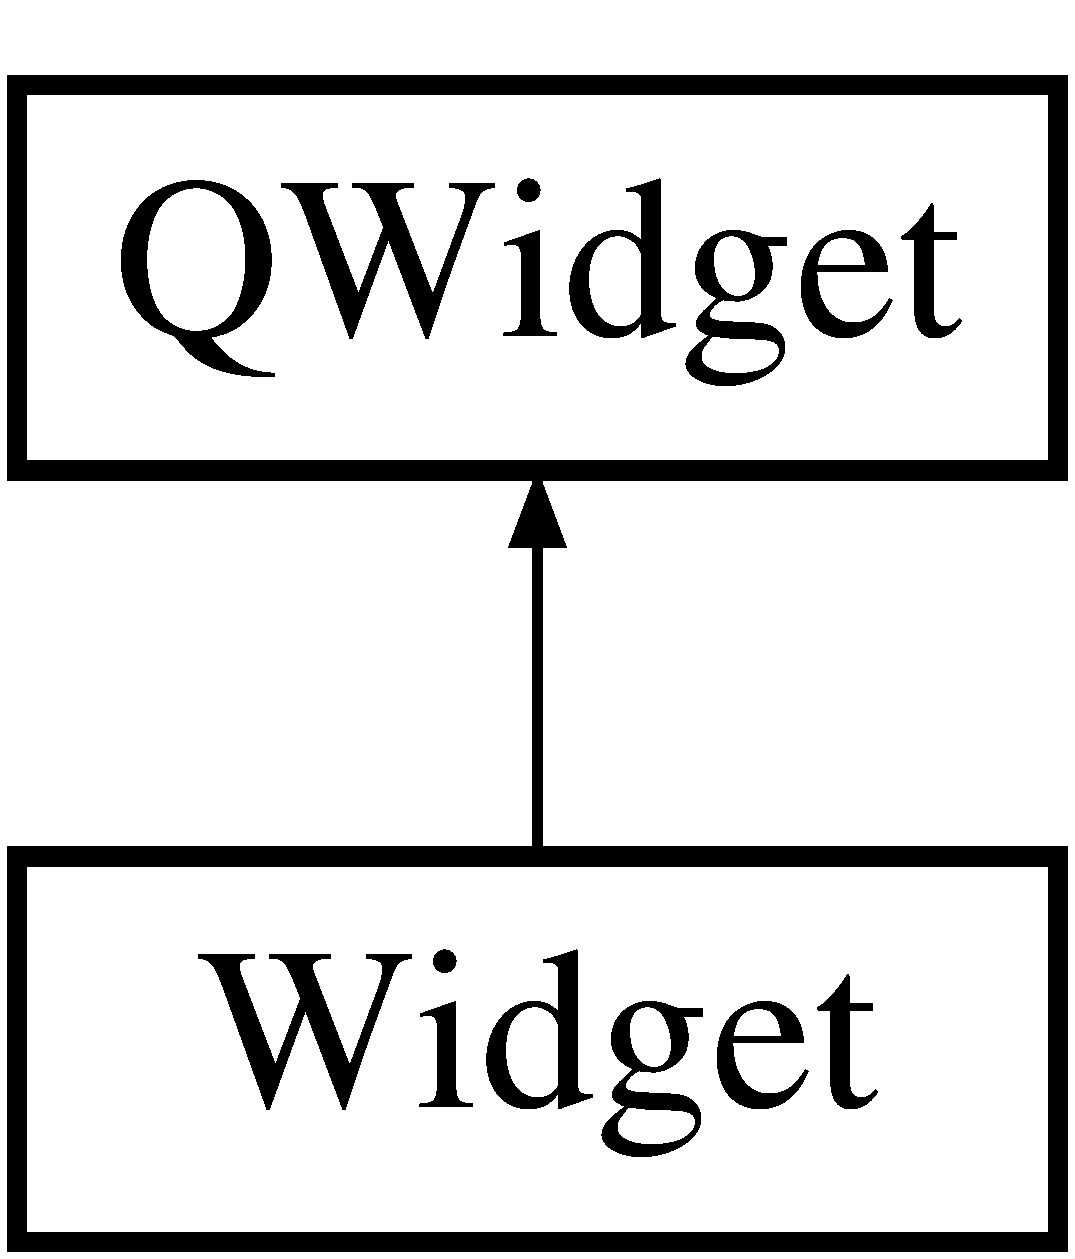
\includegraphics[height=2.000000cm]{classWidget}
\end{center}
\end{figure}
\subsection*{Public Member Functions}
\begin{DoxyCompactItemize}
\item 
\mbox{\Hypertarget{classWidget_a29531c7f141e461322981b3b579d4590}\label{classWidget_a29531c7f141e461322981b3b579d4590}} 
{\bfseries Widget} (Q\+Widget $\ast$parent=0)
\item 
\mbox{\Hypertarget{classWidget_af755e8891f462562c88c37735345a798}\label{classWidget_af755e8891f462562c88c37735345a798}} 
void {\bfseries paint\+Event} (Q\+Paint\+Event $\ast$event)
\item 
\mbox{\Hypertarget{classWidget_a1957e1c36c79f040037f4c29f2d3962d}\label{classWidget_a1957e1c36c79f040037f4c29f2d3962d}} 
void {\bfseries mouse\+Press\+Event} (Q\+Mouse\+Event $\ast$)
\item 
\mbox{\Hypertarget{classWidget_a3d9a2d8d04d59810bb619e8b1b597ba3}\label{classWidget_a3d9a2d8d04d59810bb619e8b1b597ba3}} 
void {\bfseries mouse\+Release\+Event} (Q\+Mouse\+Event $\ast$)
\item 
\mbox{\Hypertarget{classWidget_ae581766297a4d8d581ff5c24fb18707c}\label{classWidget_ae581766297a4d8d581ff5c24fb18707c}} 
void {\bfseries mouse\+Move\+Event} (Q\+Mouse\+Event $\ast$)
\item 
\mbox{\Hypertarget{classWidget_a625e5d7a5774d12c1a57fcbeb0a965ed}\label{classWidget_a625e5d7a5774d12c1a57fcbeb0a965ed}} 
void {\bfseries mouse\+Double\+Click\+Event} (Q\+Mouse\+Event $\ast$)
\item 
\mbox{\Hypertarget{classWidget_a3b087438cb505af656cb9f885681ae24}\label{classWidget_a3b087438cb505af656cb9f885681ae24}} 
void {\bfseries key\+Press\+Event} (Q\+Key\+Event $\ast$)
\item 
\mbox{\Hypertarget{classWidget_a2fcd3c4453784d68e102bbee84ed8e46}\label{classWidget_a2fcd3c4453784d68e102bbee84ed8e46}} 
void {\bfseries Show\+Context\+Menu} (const Q\+Point \&)
\end{DoxyCompactItemize}
\subsection*{Static Public Member Functions}
\begin{DoxyCompactItemize}
\item 
\mbox{\Hypertarget{classWidget_aa07cb14c8c863c9f18083be1971d7a5f}\label{classWidget_aa07cb14c8c863c9f18083be1971d7a5f}} 
static void {\bfseries clear\+Blocks} ()
\end{DoxyCompactItemize}
\subsection*{Static Public Attributes}
\begin{DoxyCompactItemize}
\item 
\mbox{\Hypertarget{classWidget_abe90e3d11863b73206f0ad77131bb25f}\label{classWidget_abe90e3d11863b73206f0ad77131bb25f}} 
static vector$<$ \hyperlink{classBlock}{Block} $\ast$ $>$ $\ast$ {\bfseries Block\+List} = new vector$<$\hyperlink{classBlock}{Block}$\ast$$>$()
\item 
\mbox{\Hypertarget{classWidget_a81c8f66ab759bc85296cd79f0657f7f4}\label{classWidget_a81c8f66ab759bc85296cd79f0657f7f4}} 
static \hyperlink{classPoint2D}{Point2D} $\ast$ {\bfseries Click\+Pos} = nullptr
\item 
\mbox{\Hypertarget{classWidget_addece0cbdceb758e88758b87e4a2dbcc}\label{classWidget_addece0cbdceb758e88758b87e4a2dbcc}} 
static \hyperlink{classBlock}{Block} $\ast$ {\bfseries Edit\+Block} = nullptr
\item 
\mbox{\Hypertarget{classWidget_ab7658893bc5ac6aaa0c98dd44f42da28}\label{classWidget_ab7658893bc5ac6aaa0c98dd44f42da28}} 
static int {\bfseries step\+Counter} = 0
\item 
\mbox{\Hypertarget{classWidget_a5c333f100a5d090ec878558fc4e9c9f8}\label{classWidget_a5c333f100a5d090ec878558fc4e9c9f8}} 
static bool {\bfseries is\+Debug} = false
\end{DoxyCompactItemize}
\subsection*{Private Slots}
\begin{DoxyCompactItemize}
\item 
\mbox{\Hypertarget{classWidget_a2e486690913bcc4df153102f30e9bbf8}\label{classWidget_a2e486690913bcc4df153102f30e9bbf8}} 
void {\bfseries Edit} ()
\item 
\mbox{\Hypertarget{classWidget_a7bfb6be2621893a32cf5a9779387d7c4}\label{classWidget_a7bfb6be2621893a32cf5a9779387d7c4}} 
void {\bfseries Delete\+Block} ()
\item 
\mbox{\Hypertarget{classWidget_aed117e0c294b2945bbcdd350721e025f}\label{classWidget_aed117e0c294b2945bbcdd350721e025f}} 
void {\bfseries Exit} ()
\end{DoxyCompactItemize}
\subsection*{Private Attributes}
\begin{DoxyCompactItemize}
\item 
\mbox{\Hypertarget{classWidget_af0e5f7d75f5c030cda9abc2c04155cb7}\label{classWidget_af0e5f7d75f5c030cda9abc2c04155cb7}} 
Q\+Painter {\bfseries painter}
\item 
\mbox{\Hypertarget{classWidget_a19c48cc897c43aa2e995fce9f7fb2418}\label{classWidget_a19c48cc897c43aa2e995fce9f7fb2418}} 
Ui\+::\+Widget $\ast$ {\bfseries ui}
\item 
\mbox{\Hypertarget{classWidget_a6122c1dcaeb90b6d84c1ed8dc3f0a60a}\label{classWidget_a6122c1dcaeb90b6d84c1ed8dc3f0a60a}} 
Q\+Rect $\ast$ {\bfseries rect}
\item 
\mbox{\Hypertarget{classWidget_a110805b026dce7cb7a0ceaac58bc46e9}\label{classWidget_a110805b026dce7cb7a0ceaac58bc46e9}} 
bool {\bfseries was\+In\+Port} = false
\item 
\mbox{\Hypertarget{classWidget_ad933df66c50281f1cae0d1f834ca5c82}\label{classWidget_ad933df66c50281f1cae0d1f834ca5c82}} 
\hyperlink{classPort}{Port} $\ast$ {\bfseries clicked\+Port} = nullptr
\item 
\mbox{\Hypertarget{classWidget_a5d74de276b9c26599037abfd60beb801}\label{classWidget_a5d74de276b9c26599037abfd60beb801}} 
\hyperlink{classLink}{Link} $\ast$ {\bfseries delete\+Link} = nullptr
\item 
\mbox{\Hypertarget{classWidget_a7d1e214005f1062688dcde868a6d40d1}\label{classWidget_a7d1e214005f1062688dcde868a6d40d1}} 
E\+Edit\+Block {\bfseries type\+Of\+Edit} = N\+O\+NE
\item 
\mbox{\Hypertarget{classWidget_a16ab9de873a36b0e0d11c19ec1f3eb45}\label{classWidget_a16ab9de873a36b0e0d11c19ec1f3eb45}} 
\hyperlink{classPoint2D}{Point2D} $\ast$ {\bfseries end\+Drag} = nullptr
\item 
\mbox{\Hypertarget{classWidget_a4fc5106cbb60fdcb49f5d003c3ed2f40}\label{classWidget_a4fc5106cbb60fdcb49f5d003c3ed2f40}} 
Q\+Menu {\bfseries my\+Menu}
\end{DoxyCompactItemize}


The documentation for this class was generated from the following files\+:\begin{DoxyCompactItemize}
\item 
widget.\+h\item 
widget.\+cpp\end{DoxyCompactItemize}

%--- End generated contents ---

% Index
\backmatter
\newpage
\phantomsection
\clearemptydoublepage
\addcontentsline{toc}{chapter}{Index}
\printindex

\end{document}
